% ======================================================================
%  DataPowerChords — Project Report (SINGLE-FILE VERSION)
%  HSLU Data Warehouse & Data Lake semester project, 2026
%  Submission: 2026-06-07 23:55
%
%  Overleaf setup:
%   1. New Project -> Blank Project
%   2. Delete default main.tex content, paste THIS ENTIRE FILE in
%   3. Compiler: pdfLaTeX
%   4. Recompile (twice — second pass resolves internal references)
%
%  Ownership per section:
%     Sec 1 Introduction        — S2 + S3 (primary); S1 methodology paragraph
%     Sec 2 Data Lake           — S1 (primary); S2 + S3 domain assumptions
%     Sec 3 Data Ingestion      — S2 (primary); S1 + S3 per-domain subsections
%     Sec 4 Data Storage        — S1 (primary); S2 + S3 domain DB designs
%     Sec 5 Data Transformation — S3 (primary); S1 + S2 per-domain subsections
%     Sec 6 Data Warehouse      — S2 (primary); S1 + S3 domain schema contrib.
%     Sec 7 Data Visualization  — S3 (primary); S1 + S2 research-question answers
%     Sec 8 Conclusions         — all three (equal split)
%
%  Search for "TODO" to find your writing assignments.
%  Remove \usepackage{lipsum} + all \lipsum[...] calls before final submission.
% ======================================================================

\documentclass[11pt,a4paper]{article}

% ----- Core packages -----
\usepackage[utf8]{inputenc}
\usepackage[T1]{fontenc}
\usepackage[english]{babel}
\usepackage[a4paper,
            top=2.8cm, bottom=2.8cm, left=3cm, right=2.8cm,
            headheight=14pt]{geometry}

% ----- Academic typography -----
% Latin Modern Roman — serif body font, LaTeX's standard academic face.
% Replace with `\usepackage{newtxtext,newtxmath}` for Times New Roman style,
% or `\usepackage{mathpazo}` for Palatino, if preferred.
\usepackage{lmodern}
\usepackage{microtype}            % subtle character protrusion + font expansion
\usepackage{setspace}             % for \onehalfspacing below
\usepackage{indentfirst}          % indent the first paragraph after each heading
\usepackage{amsmath}
\usepackage{amssymb}
\usepackage{textcomp}
\usepackage{csquotes}              % proper English quotation marks
\usepackage{lipsum}                % placeholder text; remove before final submission

% Line spacing: one-and-a-half is the academic report standard.
% For a thesis-like double spacing, use \doublespacing instead.
\onehalfspacing

% Classic academic paragraphs: indented first line, no vertical gap between.
\setlength{\parindent}{1.2em}
\setlength{\parskip}{0pt}

% ----- Layout & typography -----
\usepackage{graphicx}
\usepackage{booktabs}
\usepackage{tabularx}
\usepackage{array}
\usepackage{xcolor}
\usepackage{enumitem}
\usepackage{titlesec}
\usepackage{float}

% Captions: small, bold label, italic body — a clean academic style.
\usepackage[font=small,labelfont=bf,textfont=it,
            justification=centering,labelsep=period]{caption}

% Running header: chapter/section on the left, page number on the right.
\usepackage{fancyhdr}
\pagestyle{fancy}
\fancyhf{}
\renewcommand{\headrulewidth}{0.4pt}
\fancyhead[L]{\small\itshape\nouppercase{\leftmark}}
\fancyhead[R]{\small\thepage}
\fancypagestyle{plain}{%
  \fancyhf{}%
  \fancyfoot[C]{\small\thepage}%
  \renewcommand{\headrulewidth}{0pt}%
}

% ----- Code listings -----
\usepackage{listings}
\definecolor{codegray}{rgb}{0.95,0.95,0.95}
\definecolor{codekey}{rgb}{0.1,0.2,0.7}
\definecolor{codecomment}{rgb}{0.1,0.5,0.1}
\lstset{
  backgroundcolor=\color{codegray},
  basicstyle=\ttfamily\footnotesize,
  keywordstyle=\color{codekey}\bfseries,
  commentstyle=\color{codecomment}\itshape,
  breaklines=true,
  showstringspaces=false,
  frame=single,
  framerule=0pt,
  numbers=none,
  aboveskip=1em,
  belowskip=1em
}

% ----- Custom colors (defined before hyperref uses them) -----
\definecolor{hslublue}{RGB}{0,73,144}

% ----- Links & references -----
% xurl allows line breaks at ANY character inside URLs (not just hyphens).
% This prevents long URLs from running past the right margin.
\usepackage{xurl}
\usepackage[colorlinks=true,
            linkcolor=hslublue,
            urlcolor=hslublue,
            citecolor=hslublue,
            breaklinks=true,
            pdftitle={Geopolitics Meets Oil Markets: A Data Lake Approach to Analyzing Conflict-Driven Price Movements}]{hyperref}

\usepackage{tikz}
\usetikzlibrary{arrows.meta, positioning, shapes.geometric, fit, backgrounds}

% ----- Text wrapping safety net -----
% emergencystretch lets LaTeX loosen word spacing a little rather than produce
% overfull hboxes. tolerance raises the threshold for acceptable line breaks.
\setlength{\emergencystretch}{3em}
\tolerance=1000
\hbadness=2000       % suppress "underfull hbox" warnings below this badness

% Explicit hyphenation hints for project-specific terms that LaTeX cannot
% break on its own. Add more here if overfull warnings mention specific words.
\hyphenation{%
  Data-Power-Chords
  Alpha-Vantage
  data-ware-house
  data-base
  Post-gre-SQL
  Event-Bridge
  Cloud-Watch
  Secrets-Manager
  Step-Functions
}

% ----- Section headings -----
% Section: HSLU blue for top level (matches institutional template).
% Subsection / subsubsection: black serif — more restrained, more academic.
\titleformat{\section}
  {\Large\bfseries\color{hslublue}}{\thesection}{0.75em}{}
\titleformat{\subsection}
  {\large\bfseries}{\thesubsection}{0.75em}{}
\titleformat{\subsubsection}
  {\normalsize\bfseries\itshape}{\thesubsubsection}{0.75em}{}
\titlespacing*{\section}{0pt}{2.5ex plus 1ex minus .2ex}{1.5ex plus .2ex}
\titlespacing*{\subsection}{0pt}{2ex plus 1ex minus .2ex}{1ex plus .2ex}
\titlespacing*{\subsubsection}{0pt}{1.5ex plus 1ex minus .2ex}{0.8ex plus .2ex}

% ----- Project metadata (fill in before submission) -----
\newcommand{\projecttitle}{Geopolitics Meets Oil Markets: A Data Lake Approach to Analyzing Conflict-Driven Price Movements}
\newcommand{\groupname}{DataPowerChords}
\newcommand{\studentone}{S~1 Kethrin Heinze, Matriculation~\#18-678-680, kethrin.heinze@stud.hslu.ch}
\newcommand{\studenttwo}{S~2 Valeska Blank, Matriculation~\#01-297-738, valeska.blank@stud.hslu.ch}
\newcommand{\studentthree}{S~3 Simon Ziegs, Matriculation~\#18-731-588, simon.ziegs@stud.hslu.ch}
\newcommand{\examinerone}{PD Dr. Luis Terán}
\newcommand{\examinertwo}{José Mancera}
\newcommand{\examinerthree}{Dr. Jhonny Pincay}
\newcommand{\githuburl}{\url{https://github.com/Valeska1979/data-lake-dwh-project}}
\newcommand{\vizurl}{\url{https://public.tableau.com/...}}
\newcommand{\submissiondate}{Luzern, 7 June 2026}

% ======================================================================
\begin{document}
% ======================================================================

% ---------- Title page ----------
\begin{titlepage}
  \begin{flushleft}
    \textbf{\huge HSLU}\\[0.1em]
    {\large Hochschule Luzern}\\
    {\large Lucerne University of Applied Sciences and Arts}
  \end{flushleft}

  \vspace{4cm}
  \begin{center}{\LARGE \textbf{\projecttitle}}\end{center}
  \vspace{2cm}

  \begin{center}
  \begin{tabular}{r l}
    \textbf{Group Name:}  & \groupname \\
    \textbf{Students:}    & \studentone \\
                          & \studenttwo \\
                          & \studentthree \\[1em]
    \textbf{Examiners:}   & \examinerone \\
                          & \examinertwo \\
                          & \examinerthree \\
  \end{tabular}
  \end{center}

  \vspace{2cm}
  \begin{center}
    \textbf{GitHub:} \githuburl \\[0.3em]
    \textbf{Visualization / Demo:} \vizurl
  \end{center}

  \vfill
  \begin{center}\submissiondate\end{center}
\end{titlepage}

% ---------- Front matter ----------
\pagenumbering{roman}
\tableofcontents
\newpage
\pagenumbering{arabic}
\setcounter{page}{1}

% ======================================================================
% SECTION 1 — PROJECT IDEA AND USE CASE
% Primary authors: S2 + S3 (already drafted)
% Contributor:     S1 (methodology paragraph in 1.3.1)
% ======================================================================

\section{Project Idea and Use Case}
\label{sec:introduction}

\subsection{Topic Introduction (S2 + S3)}
\label{sec:topic_introduction}

% TODO S2/S3: Topic intro — Middle East conflict (Iran focus) impact on oil
% markets and oil-company stocks, with news sentiment as a predictive overlay.

Geopolitical tensions in the Middle East continue to play a critical role in shaping global financial markets. In the last months, the impact of the Iran conflict on oil prices and stock markets has become a persistent theme in international news coverage. Recent developments, including the escalation of the Iran war in March and April 2026, have been associated with sharp reactions in crude oil markets, renewed volatility in equity markets, and major concerns about supply disruptions through the Strait of Hormuz.  

Despite these visible market reactions, the relationship between geopolitical events and financial market dynamics remains complex and difficult to quantify. While it is generally assumed that conflicts and escalations lead to increases in oil prices, the extent to which equity markets, particularly major oil and energy companies, respond in a similar or divergent way is less clear. Additionally, the role of news sentiment and different types of geopolitical events in driving market behavior is not fully understood.  

This project addresses this challenge by designing and implementing a cloud-based data pipeline to analyze the impact of Middle Eastern geopolitical events on both oil prices and energy sector stocks. The pipeline integrates multiple data sources, including oil price data (Brent and WTI), stock price data of major oil and energy companies, real-time news data with sentiment information, and AI-generated classifications of geopolitical events. Using a data lake and data warehouse architecture, the project enables the structured collection, storage, and analysis of heterogeneous data in a scalable and reproducible way. 

The relevance of this topic lies in both its economic importance and its technical implications. From a business perspective, understanding how geopolitical events influence oil prices and related stock markets is highly valuable for commodity traders, financial analysts, and geopolitical risk experts. From a technical perspective, the project demonstrates how modern cloud technologies can be used to build an end-to-end data pipeline that supports data ingestion, enrichment, and analysis across multiple data domains. By combining real-world events with structured market data, the project provides a practical framework for analyzing complex relationships in dynamic market environments.

\subsection{Motivation (S2 + S3)}
\label{sec:motivation}

% TODO S2/S3: Motivation — why this project, why now.

This project is motivated by the strong and ongoing influence of geopolitical developments in the Middle East on global financial markets. Events involving Iran, such as sanctions, military escalations, uncertainty and rapidly changing conditions regarding the status of the Strait of Hormuz, or diplomatic negotiations, are regularly associated with sudden changes not only in oil prices but also in the stock prices of major oil and energy companies. Given the economic importance of both commodity markets and equity markets, understanding these relationships is of high relevance for market participants, analysts, and even consumers, as fluctuations in oil prices are directly reflected in retail fuel prices.  

In addition to its economic significance, the topic provides a suitable use case for applying concepts from the Data Lakes and Data Warehouses module. The integration of heterogeneous data sources, including oil price data, stock market data, news data with sentiment information, and AI-generated event classifications, enables the analysis of complex relationships between geopolitical events and different segments of financial markets. Such a setup reflects real-world analytical challenges, where data is distributed across multiple sources, formats, and domains. 

Furthermore, the project enables the practical implementation of a cloud-based data pipeline using modern technologies. By combining data ingestion, storage, transformation, and analysis within a unified architecture, it is demonstrated how scalable and automated systems can be built to support data-driven insights across multiple asset classes. This makes the topic not only relevant from a business perspective but also valuable from a technical and educational standpoint. 

\subsection{Problem Definition and Goals}
\label{sec:problem_goals}

\subsubsection{Business and Research Questions}
\label{sec:research_questions}

The data lake implementation answers the following research questions:

\begin{enumerate}[label=\textbf{Q\arabic*.}, leftmargin=*]
  \item How do conflict-escalation events involving Iran correlate with
        short-term WTI and Brent price spikes?
  \item Do stock prices of the top oil companies move in sync during
        Iran conflict events, or do they diverge across subsectors
        (majors, E\&P, refiners, services, tankers)?
  \item Can conflict-event intensity around Iran and the Middle East
        identify oil-price volatility windows?
  \item Which event types (sanctions, military strikes, nuclear
        negotiations, Strait of Hormuz incidents) have the strongest
        and most persistent price impact?
\end{enumerate}

% TODO S1: methodology paragraph (3–5 sentences) — cross-source
% event-study design that ties stocks, oil, and news together.

\paragraph{Methodology.}
The four research questions are answered through an event-study
design [6, 7] that aligns three
independent data sources on a shared trading calendar. Stock-price
data is sourced from Yahoo Finance via the \texttt{yfinance} Python
library. The project proposal originally specified Alpha Vantage's
\texttt{TIME\_SERIES\_DAILY\_ADJUSTED} endpoint, but that endpoint
was moved to a premium tier shortly after the project began,
prompting the substitution to \texttt{yfinance}. Oil-price series are pulled
from the U.S. Energy Information Administration's open
API. Conflict event data is generated through a
Gemini-based ingestion pipeline using Google Search grounding and structured
LLM classification. The pipeline extracts and classifies Iran-region
geopolitical events into a five-category taxonomy. A conformed \texttt{dim\_date} table joins the
three domains on shared trading days, which is the precondition for
questions such as how XLE moves in the five trading days following
each Hormuz incident.

\subsubsection{Business Intelligence Questions}
\label{sec:bi_questions}

The data warehouse implementation answers the following business
intelligence questions:

\begin{enumerate}[label=\textbf{BI\arabic*.}, leftmargin=*]
  \item What is the typical magnitude and duration of WTI/Brent price
        moves in the trading days following each event category?
  \item Which oil-company subsectors are most reactive to a given event
        category, measured by idiosyncratic return?
  \item How does rolling 30-day conflict intensity correlate with
        realised and idiosyncratic volatility of the energy sector ETF
        (XLE)?
  \item Which individual events in the analysis window had the largest
        measurable price impact across both oil and equity markets?
\end{enumerate}

\newpage
% ======================================================================
% SECTION 2 — DATA LAKE
% Primary author: S1
% Contributors:   S2 (oil-source assumptions), S3 (news-source assumptions)
% ======================================================================

\section{Data Lake}
\label{sec:data_lake}

\subsection{Data Sources (S1)}
\label{sec:data_sources}

The project uses three complementary dynamic data sources.

\paragraph{Stock-price data (S1, yfinance).}
Daily Open / High / Low / Close / Volume (OHLCV) observations together
with split- and dividend-adjusted closing prices are retrieved via the
open-source \texttt{yfinance} Python library, which
provides programmatic access to Yahoo Finance's historical quotation
back-end.
The instrument universe comprises fifteen tickers selected to
represent the principal segments of the global oil-and-energy equity
complex: integrated majors (XOM, CVX, SHEL); upstream exploration and
production (COP, OXY, DVN); downstream refining (VLO, MPC); oilfield
services (SLB, HAL, BKR); tanker shipping (FRO); and sector benchmarks
(XLE, USO, SPY). The original project specification selected Alpha
Vantage's \texttt{TIME\_SERIES\_DAILY\_ADJUSTED} endpoint; this was
superseded in May 2026 after the endpoint was reclassified as
premium-tier, which rendered the free-tier assumption non-viable.
The principal limitation of \texttt{yfinance}, namely that it is an
unofficial client against an undocumented Yahoo back-end with no
service-level guarantee on schema stability, is addressed transparently
in Section~8, together with a contingency migration
path to a paid official feed.

\paragraph{Oil-price data (S2, EIA API).}
% TODO S2
Oil price data is sourced from the U.S. Energy Information Administration (EIA) API, which provides daily observations for the Brent and WTI benchmarks in a structured and machine-readable format. These benchmarks are widely recognised indicators of global oil market developments and are particularly relevant for analysing the impact of geopolitical events on energy markets. As the project aims to investigate potential relationships between Middle East conflicts and oil price movements, the data directly supports the use case by providing reliable and timely market information. Furthermore, the API enables automated data retrieval and seamless integration into a cloud-based data lake architecture, supporting scalable ingestion, storage, transformation, and downstream analytics.

\paragraph{News and classified events (S3, Gemini API).}
The original design used World News API for article retrieval and
Gemini only for classification. This was changed after implementation
testing showed that the free news-API tiers, including World News API
and comparable alternatives, did not provide enough historical depth
for the 2025--2026 event-study window. The final source is therefore
Gemini 2.5 Flash with Google Search grounding. Each Lambda invocation
asks Gemini to research Iran-region geopolitical conflict events for a
bounded weekly interval and to return a strict JSON array containing
the event date, category, severity, actors, location, short summary,
description, date confidence, and source hint. This approach keeps the
pipeline dynamic while preserving the historical coverage required by
the research questions.

\paragraph{Data Catalog.}
All tables across the bronze, silver, and gold zones are registered in
the AWS Glue Data Catalog under the database
\texttt{dwl\_datapowerchords}. Each table carries three mandatory
tags: \texttt{project}, \texttt{owner}, and \texttt{domain}.

\paragraph{Schema and Versioning Strategy.}
All silver-zone Parquet writes enforce a strict schema via PyArrow.
Schema evolution policy is additive-only: new columns are tolerated;
removed or renamed columns cause a transform failure alarmed via SNS.
The ticker dimension uses Slowly Changing Dimension Type 2 to capture
renames or delistings.

\subsection{Architecture (S1)}
\label{sec:data_lake_architecture}

The data lake is implemented on AWS in region \texttt{us-east-1}. All
resources carry cost-allocation tags for per-domain budget visibility.
Figure~1 gives the high-level layout: three
independent dynamic API sources feed a daily ingestion layer
(EventBridge $\to$ Step Functions $\to$ Lambda) that writes raw
payloads to the S3 bronze zone; transform Lambdas convert bronze into
silver and gold Parquet zones, all three of which are catalogued by
AWS~Glue; gold is served \emph{both} by Athena (the interim demo
path that de-risked the May~21 presentation and acts as the
permanent fallback if any warehouse load slips) and by
RDS~PostgreSQL after the warehouse load step (the primary serving
path for sub-second Tableau interactions).

\begin{figure}[H]
  \centering
  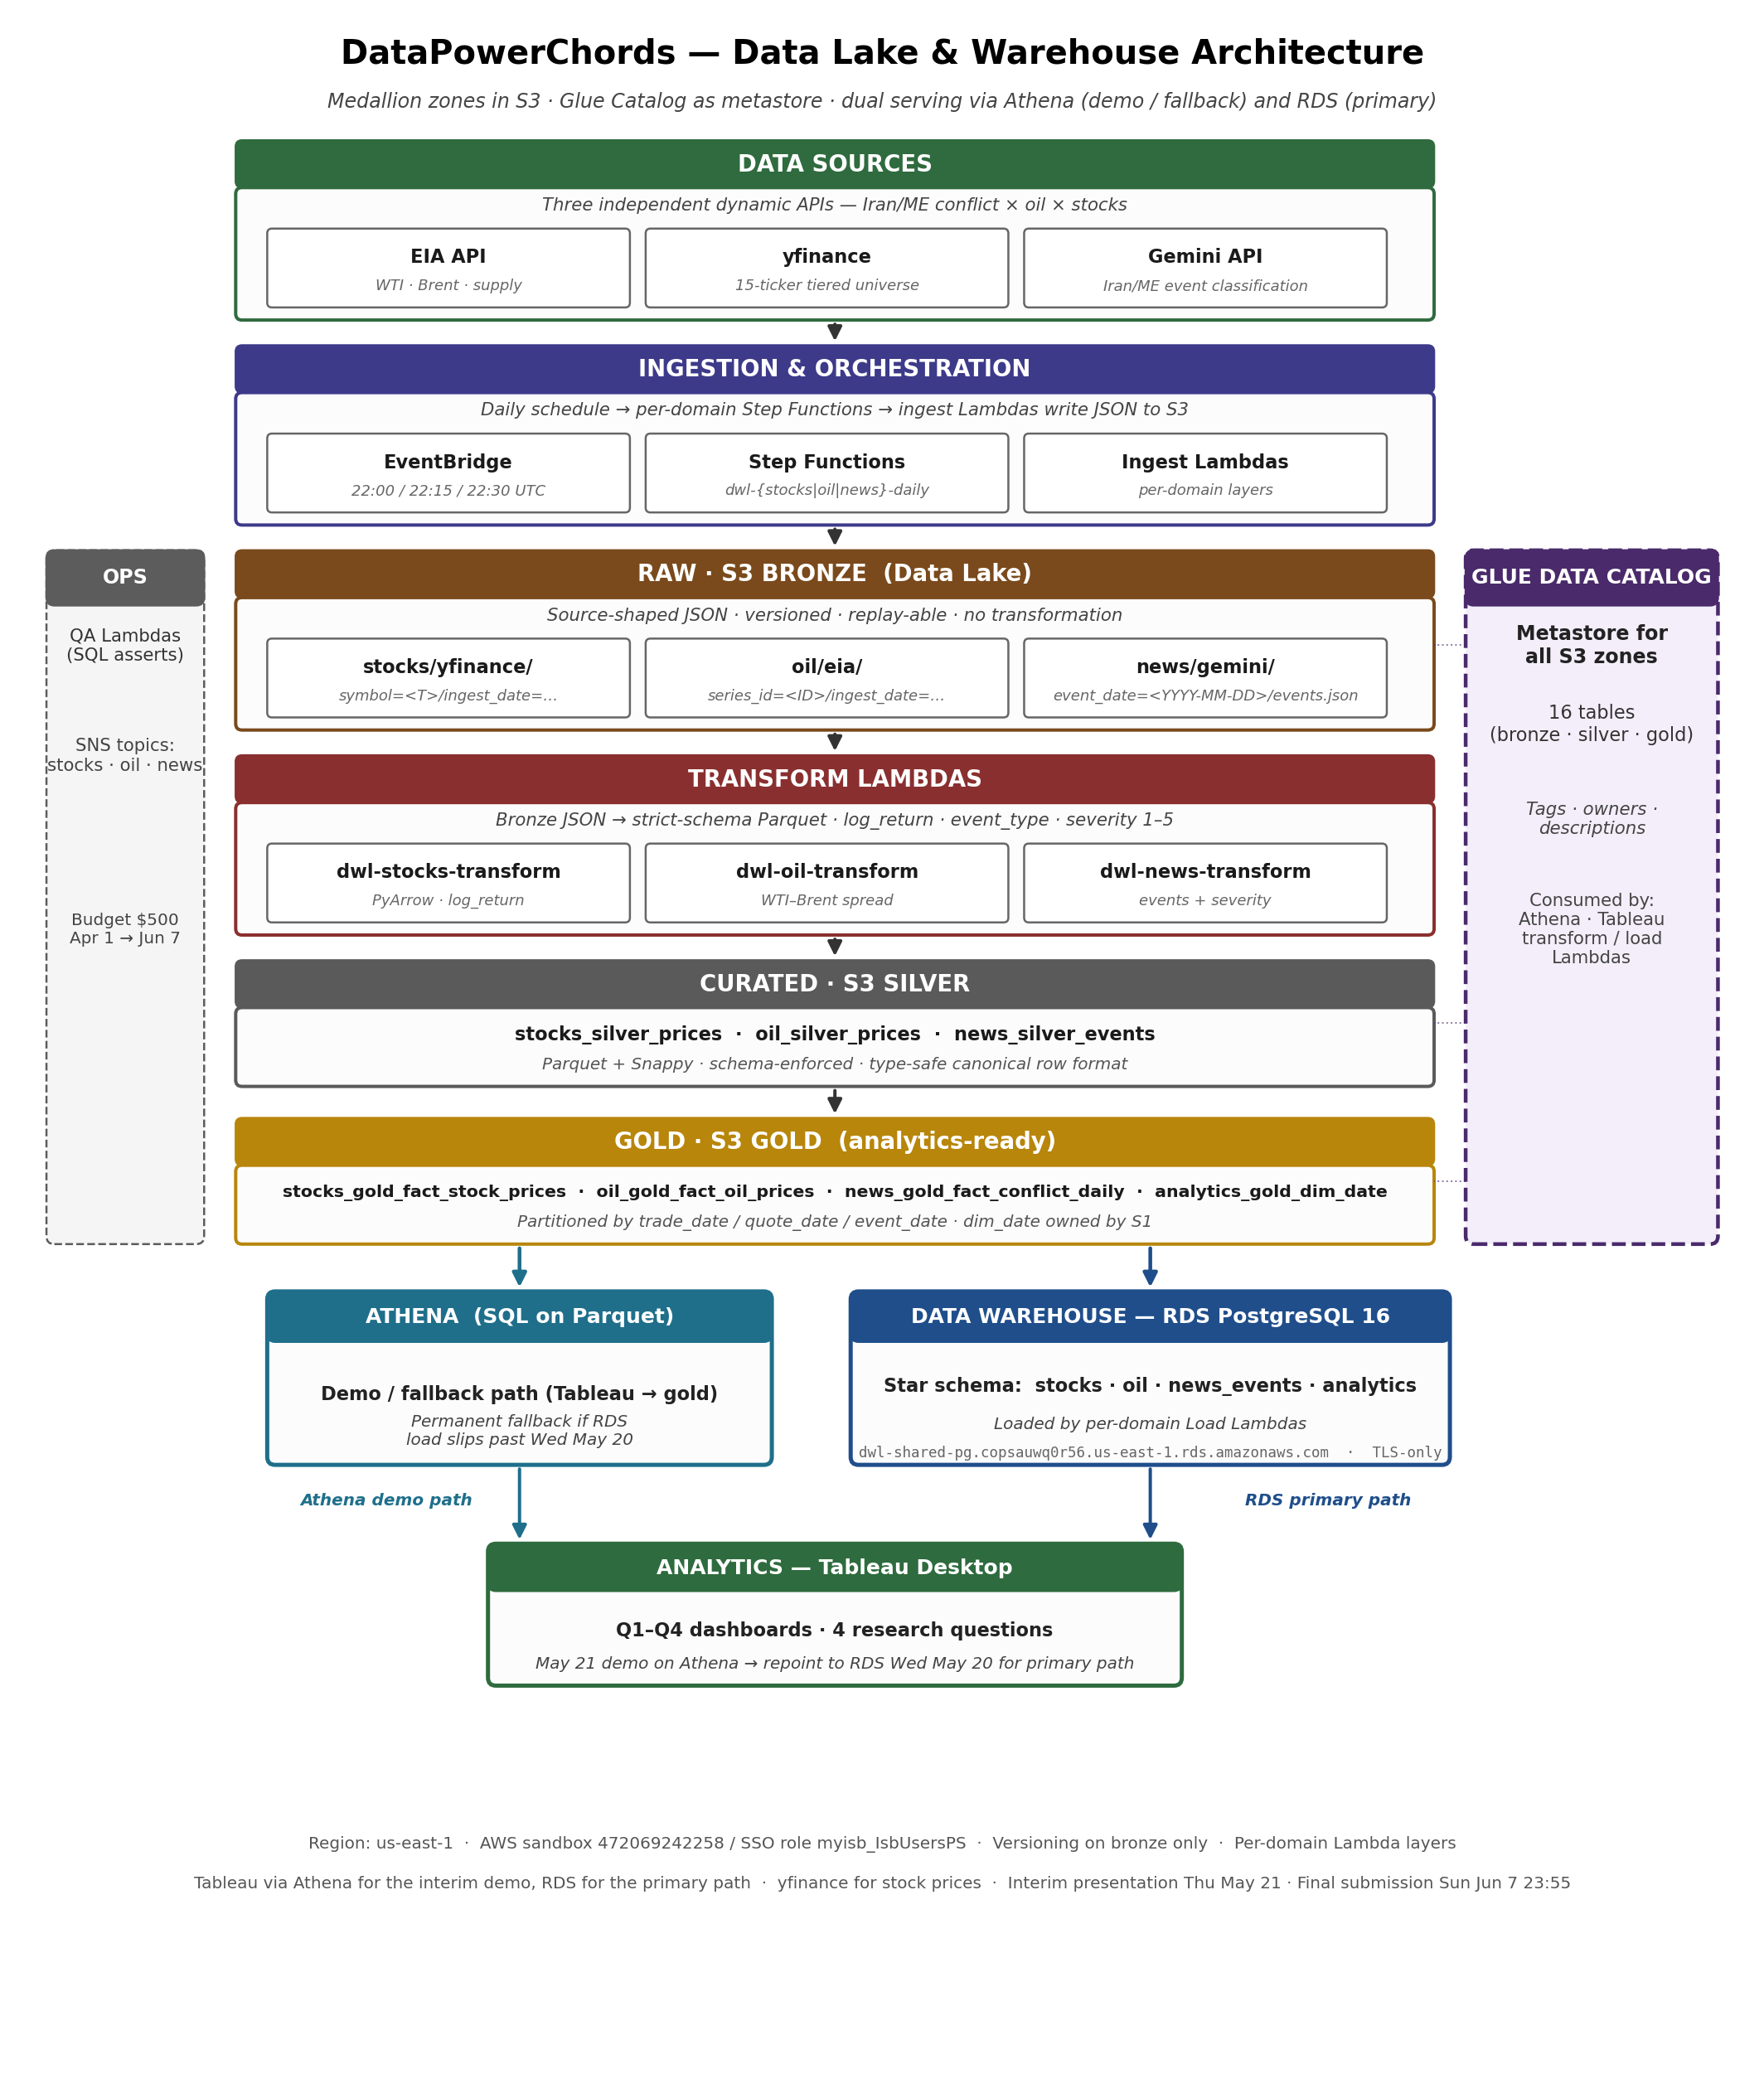
\includegraphics[width=\textwidth]{figures/architecture.png}
  \caption{End-to-end data-lake-and-warehouse architecture. The
    Glue~Data~Catalog (right sidebar) is the metastore that makes
    every S3 zone queryable. The dual Athena and RDS serving path
    at the bottom is the project's solution for keeping the lake
    queryable before the warehouse load completes
    and for the warehouse to remain the steady-state serving layer
    thereafter.}
  \label{fig:architecture}
\end{figure}

\paragraph{Cloud Infrastructure.} Core services:
\begin{itemize}
  \item Amazon S3 for zone storage (three buckets, see below).
  \item Amazon RDS for PostgreSQL~16.13 hosting the warehouse star
        schemas. The shared instance \texttt{dwl-shared-pg}
        (\texttt{db.t4g.micro}, gp3 20\,GB, Single-AZ) is publicly
        reachable so that Tableau Desktop and out-of-VPC Lambdas can
        connect; access is gated by a strong auto-generated password
        stored in AWS Secrets Manager and a custom parameter group
        \texttt{dwl-postgres16-forcessl} that sets
        \texttt{rds.force\_ssl=1}, causing the broker to reject any
        non-TLS connection attempt.
  \item AWS Lambda for serverless compute (Python~3.11 runtime,
        x86\_64 architecture). Domain-specific dependencies are
        bundled as per-domain Lambda layers rather than a single
        shared dependency layer. For the stocks domain this comprises
        \texttt{dwl-stocks-yfinance} for the ingest function and
        \texttt{dwl-stocks-deps} (containing pandas, PyArrow,
        psycopg2-binary, and requests) for the downstream transform
        and load functions. The AWS-imposed \mbox{250\,MB} unzipped
        layer-size cap on a single function precludes attaching both
        layers simultaneously, which informs the per-stage Lambda
        decomposition described in Section~3.
  \item Amazon EventBridge for daily scheduling.
  \item AWS Step Functions for orchestration with retries and DLQ.
  \item AWS Glue Data Catalog (database \texttt{dwl\_datapowerchords})
        for metadata across all 16 bronze/silver/gold tables.
  \item AWS Secrets Manager for API keys and DB credentials.
  \item Amazon SNS for alerts (one topic per domain:
        \texttt{dwl-stocks-alerts}, \texttt{dwl-oil-alerts},
        \texttt{dwl-news-alerts}); Amazon SQS as DLQ.
\end{itemize}

\paragraph{Storage Layers and Zones.}
The data lake follows a standard bronze--silver--gold pattern,
implemented as three S3 buckets in \texttt{us-east-1}, all with
Block-All-Public-Access on and SSE-S3 default encryption:
\begin{itemize}
  \item \textbf{Bronze (raw)}
        (\texttt{dwl-datapowerchords-raw}): unmodified JSON from
        each API. S3 versioning is enabled to preserve the immutable
        source of truth and to recover from accidental ingest-Lambda
        overwrites.
  \item \textbf{Silver (curated)}
        (\texttt{dwl-datapowerchords-curated}): Snappy-Parquet with
        strict schema. S3 versioning is disabled because silver is
        deterministically rebuildable from raw via re-running the
        transform Lambdas.
  \item \textbf{Gold (analytics-ready)}
        (\texttt{dwl-datapowerchords-gold}): Parquet partitioned
        by date. S3 versioning is disabled for the same reason as
        silver.
\end{itemize}

\paragraph{File Formats.}
JSON is used for bronze to preserve full response fidelity. Parquet
with Snappy compression is used for silver and gold because the
dominant query pattern is columnar scan across tickers for a date
range, which Parquet serves efficiently.

\paragraph{Streaming vs Batch.}
All ingestion is daily batch triggered by EventBridge after the US
market close (22:00 UTC, Mon--Fri). Streaming was rejected as
unnecessary overhead.

\paragraph{Network access and identity model.}
The shared RDS instance is reachable on its public DNS endpoint
(TCP~5432) gated by a single security group
\texttt{dwl-shared-rds-sg} with one inbound rule (PostgreSQL 5432 from
\texttt{0.0.0.0/0}) and forced TLS at the broker level. There is no
NAT gateway, no VPN, and no PrivateLink, which realises the project's
chosen posture of a public RDS endpoint defended by a security group,
TLS enforcement, and a strong auto-generated master password. The
trade-off is documented in Section~8:
keeping the network surface flat saves about \$30/month in NAT
gateway charges and removes a class of VPC mis-configurations, at the
cost of relying entirely on \texttt{rds.force\_ssl=1}, deletion
protection, and the auto-rotated master password to defend the public
endpoint.

The IAM identity model is shaped by the constraint of a single shared
SSO role across the team: there are no per-student IAM users in the
AWS account. All three students sign in via the HSLU
access portal and assume the same SSO permission set
(\texttt{myisb\_IsbUsersPS}); the only IAM identities the team creates
are three Lambda execution roles
(\texttt{dwl-stocks-lambda-role}, \texttt{dwl-oil-lambda-role},
\texttt{dwl-news-lambda-role}). Each Lambda role carries the AWS-managed
\texttt{AWSLambdaBasicExecutionRole} policy plus a
\texttt{dwl-<domain>-lambda-inline} policy scoped to its own domain's
S3~prefixes, Secrets~Manager namespace, SNS~alerts topic, and Glue
catalog tables, plus read access to the shared RDS master-credentials
secret. CloudTrail attributes every human action to the shared SSO
role; team-level attribution falls back to git commit history.

\paragraph{Interoperability with the Data Warehouse.}
Gold-zone tables are mirrored into the RDS PostgreSQL warehouse via
idempotent \texttt{INSERT \dots ON CONFLICT \dots DO UPDATE} upserts.
The architecture figure introduced earlier in this section
(Figure~1) shows the two serving paths from
gold: Athena directly against S3 Parquet, and RDS after the
warehouse load step.

\newpage
% ======================================================================
% SECTION 3 — DATA INGESTION
% Primary author: S2 (overall + oil subsection)
% Contributors:   S1 (AV subsection), S3 (news + Gemini subsection)
% ======================================================================

\section{Data Ingestion}
\label{sec:data_ingestion}

All three data sources are dynamic APIs accessed over HTTPS. Ingestion
follows a common pattern: an EventBridge rule triggers a per-domain
Lambda, which retrieves the source API key from Secrets Manager,
issues the necessary API calls with exponential backoff on transient
failures, and writes unmodified JSON to the bronze S3 prefix.

\subsection{Data Source Documentation}
\label{sec:data_source_doc}

\subsubsection{yfinance: Stock Prices (S1)}
\label{sec:yfinance_source}

\paragraph{Source type.}
Open-source Python library (\texttt{yfinance}, version~1.2.0)
wrapping Yahoo Finance's historical quotation back-end. The library
returns a structured pandas DataFrame at the call site rather than a
raw HTTP response, which compresses the bronze-to-silver
transformation by removing one parsing stage.

\paragraph{Library invocation.}
Each ticker is queried via the call
\texttt{yf.\allowbreak Ticker(symbol).\allowbreak history(start=start\_date,\allowbreak{} auto\_adjust=False)}.
The returned DataFrame is indexed by trading date and exposes nine
attributes per observation: \texttt{Open}, \texttt{High}, \texttt{Low},
\texttt{Close}, \texttt{Adj~Close}, \texttt{Volume}, \texttt{Dividends},
and \texttt{Stock~Splits}. The flag \texttt{auto\_adjust=False} is
required to preserve both the raw and split/dividend-adjusted closing
prices: the adjusted series supports the log-return computation in the
silver zone, while the raw close enables validation of the adjusted
series against published OHLC data.

\paragraph{Authentication.}
None. The library targets Yahoo's public unauthenticated quotation
feed, eliminating the need for API-key management in Secrets~Manager
for this domain. The Secrets~Manager entry
\texttt{dwl/stocks/alphavantage} provisioned during the initial
shared-infrastructure build against the original Alpha Vantage
specification is retained but unreferenced and is scheduled for
removal in the final cleanup pass before submission.

\paragraph{Rate limits.}
Yahoo Finance does not publish rate limits on the unauthenticated
quotation feed. Community-reported throttling thresholds, on the order
of several hundred requests per minute per source IP, are well above
this study's operating volume of fifteen requests per business
day. No client-side back-off logic is therefore implemented in the
ingest handler; transient network-level failures are handled by
yfinance's internal HTTP client (\texttt{curl\_cffi}).

\paragraph{Pagination.}
Not applicable. A single library call returns the complete date range
specified by the \texttt{start} parameter. For the project's analysis
window of 1~January~2025 to the present, the response contains
approximately 333~records per ticker, well within Lambda memory and
S3 payload bounds.

\paragraph{Implementation.}
The ingest function \texttt{dwl-stocks-ingest} is implemented as a
single Python~3.11 AWS~Lambda (architecture x86\_64,
\mbox{512\,MB} of memory, five-minute timeout). It executes under the
dedicated execution role \texttt{dwl-stocks-lambda-role}, whose
inline policy is scoped to the stocks-domain S3 prefix, the
\texttt{dwl/stocks/*} Secrets~Manager namespace, the shared
RDS master-credentials secret, and the \texttt{dwl-stocks-alerts} SNS
topic. The yfinance dependency tree is provided through the dedicated
Lambda layer \texttt{dwl-stocks-yfinance:2}, the second version of
which retains the \texttt{*.dist-info} directories required by
\texttt{importlib.metadata} for runtime introspection of \texttt{curl\_cffi}'s
own version. The handler iterates over the fifteen-ticker universe,
retrieves the historical series, normalises the column identifiers to
lowercase snake-case, and writes one JSON document per ticker per
ingestion date to the bronze prefix
\path{s3://dwl-datapowerchords-raw/stocks/yfinance/symbol=<TICKER>/ingest_date=<YYYY-MM-DD>/daily.json}.
The bronze JSON document conforms to the schema $\{\texttt{meta},
\texttt{rows}\}$, in which the \texttt{meta} object records the symbol,
ingestion date, start date, source identifier, and row count for
lineage purposes, and \texttt{rows} is an array of per-day
observations. Two operating modes are supported via the event payload.
The default \emph{routine} mode fetches a seven-day look-back, sized
to recover from any missed scheduled executions without redundantly
re-fetching the full history. The \emph{backfill} mode, triggered by
the payload \texttt{\{"backfill": true\}}, fetches the complete
historical window from the environment variable \texttt{BACKFILL\_START}
(default \texttt{2025-01-01}) and is intended for the initial seed and
for one-off catch-up runs. Daily execution is orchestrated by Amazon
EventBridge Scheduler (schedule \texttt{dwl-stocks-daily-22utc}, cron
expression \texttt{0 22 ? * MON-FRI *} in UTC) at 22:00\,UTC on US
trading days, providing a one-hour buffer after the New York Stock
Exchange close to allow the upstream feed to settle. Failures
re-attempt up to three times with a maximum event age of sixty
minutes; persistent failures are routed to the \texttt{dwl-stocks-alerts}
SNS topic for human follow-up. The bronze table is registered in the
AWS~Glue Data Catalog as
\texttt{dwl\_datapowerchords.stocks\_bronze\_yfinance} via an
on-demand crawler (\texttt{dwl-stocks-bronze-yfinance-crawler}),
partitioned by symbol and ingestion date.

\paragraph{Justification of use.}
\texttt{yfinance} was adopted after the project's originally
specified data source, Alpha~Vantage's
\texttt{TIME\_SERIES\_DAILY\_ADJUSTED} endpoint, was reclassified as
premium-tier after the project's kickoff. The reclassification
invalidated the free-tier assumption underpinning the original
selection. Among the available free-of-charge alternatives
(Polygon.io, Finnhub, Twelve Data), \texttt{yfinance} was selected on
the basis of three considerations: (i)~its established adoption in
the academic and personal quantitative-finance community, which
provides implicit social validation of data quality at the scope
required for this study; (ii)~the absence of API-key management
overhead, which removes one moving part from the security surface;
and (iii)~its native return of pandas DataFrames, which shortens the
bronze-to-silver normalisation logic in the transform stage.

\paragraph{Limitations.}
The principal acknowledged limitation is that yfinance is an
unofficial client against an undocumented Yahoo back-end and provides
no service-level guarantee against schema or availability changes.
This risk is structurally mitigated in two ways. First, the historical
window required by this study has been retrieved in full and persisted
to the immutable bronze zone (with S3 versioning enabled on the raw
bucket), so any future yfinance disruption affects only the daily
incremental
update rather than the analysis itself. Second, a contingency
migration path to a paid official feed (Polygon.io is the leading
candidate on price--quality grounds) is documented in
Section~8 as future work; because the bronze JSON
schema $\{\texttt{meta}, \texttt{rows}\}$ is independent of the
underlying source, such a migration would be confined to the ingest
handler and would not propagate downstream.

\subsubsection{EIA: Oil Prices (S2)}
\label{sec:eia_source}

\paragraph{Source type.} Dynamic REST API (EIA v2), JSON response.

\paragraph{API invocation.}
Data is retrieved from the EIA v2 API using HTTPS requests. The project queries the Brent and WTI crude oil benchmark series and receives daily price observations in JSON format. The response contains the observation date, benchmark identifier, and price value.

\paragraph{Authentication.}
API access requires an EIA API key. The key is stored securely in AWS Secrets Manager and retrieved by the ingestion Lambda at runtime.

\paragraph{Rate limits.}
The EIA API is designed for public access and supports the low request volume required by this project. The pipeline performs only a small number of requests per day, remaining well below published usage limits.

\paragraph{Pagination.}
Not applicable. The requested historical data range is returned within a single API response and does not require pagination handling.

\paragraph{Implementation.}
Oil-price ingestion is implemented as an AWS Lambda function \texttt{dwl-oil-ingest} that retrieves Brent and WTI benchmark data from the EIA API and stores the raw JSON responses in the bronze layer of the data lake. The data is subsequently transformed into curated Parquet datasets in the silver layer and integrated into the gold-layer fact table \texttt{oil.fact\_prices}. Daily execution is orchestrated through Amazon EventBridge, enabling automated ingestion and updates without manual intervention. The resulting datasets are registered in the AWS Glue Data Catalog and are accessible through Amazon Athena and the downstream data warehouse.

\paragraph{Justification of use.}
Brent and WTI are the most widely used global oil-price benchmarks and are therefore highly relevant for analysing the impact of geopolitical events on energy markets. The EIA API was selected because it provides reliable, authoritative, machine-readable data from a governmental source and integrates well into an automated cloud-based data pipeline.

\paragraph{Limitations.}
The dataset contains daily observations only. Consequently, intraday market reactions and short-term price volatility cannot be captured.

\subsubsection{Gemini Conflict Event Source (S3)}
\label{sec:news_source}

\paragraph{Source type.} Dynamic REST API call to Gemini 2.5 Flash
with Google Search grounding. Gemini is used as the event-research
source and as the classifier.

\paragraph{Query design.}
The ingest Lambda \texttt{dwl-conflict-ingest} processes the requested
analysis period in weekly chunks. The prompt constrains the scope to
Iran, Iranian state or proxy actors, and oil-market-relevant Middle
East locations including the Strait of Hormuz, Persian Gulf, Red Sea,
Iraq, Yemen, Israel, Lebanon, Syria, and Gulf states. For each week it
requests at most fifteen significant events and requires a JSON-only
response. Routine operation fetches the seven days ending yesterday;
backfill mode accepts explicit \texttt{start\_date} and
\texttt{end\_date} values.

\paragraph{Event taxonomy.}
Gemini classifies each event into one of five categories:
\texttt{sanctions}, \texttt{military\_conflict},
\texttt{security\_incidents}, \texttt{nuclear\_diplomacy}, and
\texttt{diplomatic\_shifts}. It also assigns severity on a 1--5
scale, where 1 is routine and 5 represents extreme regional-war,
Hormuz-closure, direct Iran--US/Iran--Israel, or nuclear-escalation
events.

\paragraph{Justification of use.}
The Gemini-only design was selected after the planned World News API
source proved unsuitable for historical backfill on the free tier.
Grounded Gemini calls retain a dynamic source interface, provide
historical recall across the full project window, and return the
classification fields directly in the structure needed by the lake.
The main trade-off is that source extraction and classification are
performed by a generative model, so the pipeline records
\texttt{source\_hint}, \texttt{date\_confidence}, and severity and
filters lower-confidence records before gold aggregation.

\paragraph{Limitations and mitigations.}
Using Gemini as a grounded event source introduces model-risk that is
different from a conventional news API: relevant events can be missed,
summaries can be compressed too aggressively, and categories or
severity levels can be misassigned. The implementation mitigates this
by forcing a strict JSON schema, a fixed five-category taxonomy, a
bounded weekly query window, and deterministic validation in the ingest
Lambda. Event-level records remain in silver Parquet with
\texttt{source\_hint} and \texttt{date\_confidence} for auditability,
while gold excludes approximate-date events and severity-1 routine
events so the warehouse is driven by higher-confidence conflict
signals.

\subsection{Pipeline Design}
\label{sec:pipeline_design}

All three domains use the same orchestration pattern: an EventBridge
rule triggers a Step Functions state machine that invokes ingest,
transform, load, and quality-check Lambdas in sequence. Retries are
three attempts with exponential backoff (2s, 4s, 8s); failures
ultimately land in an SNS topic and an SQS dead-letter queue.

\begin{figure}[H]
  \centering
  \resizebox{\textwidth}{!}{%
  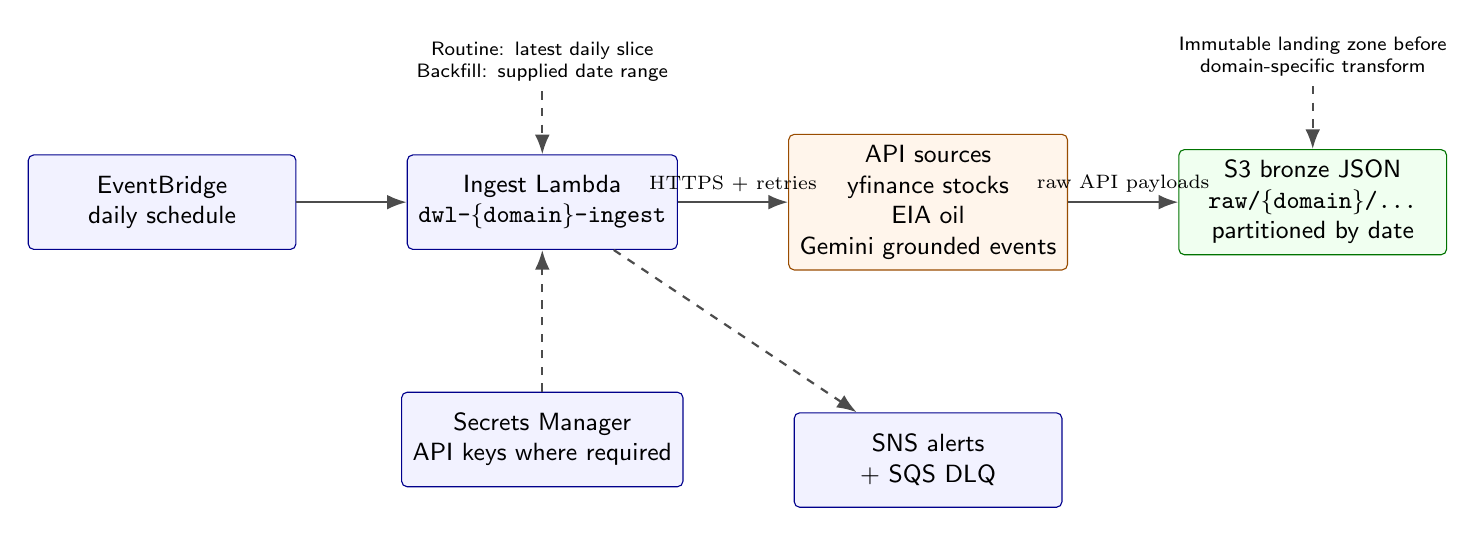
\begin{tikzpicture}[
    font=\sffamily\small,
    node distance=12mm and 14mm,
    box/.style={
      draw,
      rounded corners=2pt,
      align=center,
      minimum width=34mm,
      minimum height=12mm,
      inner sep=4pt,
      fill=white
    },
    aws/.style={
      box,
      fill=blue!5,
      draw=blue!55!black
    },
    data/.style={
      box,
      fill=green!6,
      draw=green!45!black
    },
    source/.style={
      box,
      fill=orange!8,
      draw=orange!60!black
    },
    db/.style={
      cylinder,
      draw=purple!55!black,
      fill=purple!6,
      shape border rotate=90,
      aspect=0.25,
      align=center,
      minimum width=31mm,
      minimum height=15mm,
      inner sep=4pt
    },
    note/.style={
      align=center,
      font=\sffamily\scriptsize,
      text width=34mm
    },
    arrow/.style={
      -{Latex[length=2.5mm]},
      thick,
      draw=black!70
    }
  ]

    % Main ingestion pipeline
    \node[aws] (eventbridge) {EventBridge\\daily schedule};
    \node[aws, right=of eventbridge] (ingest) {Ingest Lambda\\\texttt{dwl-\{domain\}-ingest}};
    \node[source, right=of ingest] (apis) {API sources\\yfinance stocks\\EIA oil\\Gemini grounded events};
    \node[data, right=of apis] (bronze) {S3 bronze JSON\\\texttt{raw/\{domain\}/...}\\partitioned by date};

    % Support services
    \node[aws, below=18mm of ingest] (secrets) {Secrets Manager\\API keys where required};
    \node[aws, below=18mm of apis] (alerts) {SNS alerts\\+ SQS DLQ};

    % Arrows
    \draw[arrow] (eventbridge) -- (ingest);
    \draw[arrow] (ingest) -- node[above, font=\scriptsize] {HTTPS + retries} (apis);
    \draw[arrow] (apis) -- node[above, font=\scriptsize] {raw API payloads} (bronze);

    \draw[arrow, dashed] (secrets) -- (ingest);
    \draw[arrow, dashed] (ingest) -- (alerts);

    % Annotations
    \node[note, above=8mm of ingest] (modes)
      {Routine: latest daily slice\\Backfill: supplied date range};
    \draw[arrow, dashed] (modes) -- (ingest);

    \node[note, above=8mm of bronze] (fields)
      {Immutable landing zone before domain-specific transform};
    \draw[arrow, dashed] (fields) -- (bronze);

  \end{tikzpicture}%
  }
  \caption{Common API ingestion pattern used by the stocks, oil, and news domains.}
  \label{fig:ingestion_pipeline}
\end{figure}


\paragraph{Tools and technologies.}
AWS Lambda (Python 3.12), EventBridge, S3, Secrets
Manager, SNS, Glue Data Catalog.

\subsection{Data Capture \& Handling}
\label{sec:data_capture}

\paragraph{Schema evolution.}
Silver-zone writers enforce a strict PyArrow schema; additive
upstream changes tolerated, destructive changes surface as SNS
alerts.

\paragraph{Retries and error handling.}
Transient failures are handled through AWS Lambda retry mechanisms and EventBridge re-invocation policies. Execution logs are written to Amazon CloudWatch, enabling monitoring and troubleshooting. Persistent failures are routed to an SNS notification topic for operational follow-up.

\paragraph{Duplicates and late-arriving data.}
All load-to-RDS operations use \texttt{INSERT \dots ON CONFLICT \dots
DO UPDATE} keyed on the fact's natural unique key. This renders the
pipeline idempotent and accommodates upstream republications.

\newpage
% ======================================================================
% SECTION 4 — DATA STORAGE
% Primary author: S1
% Contributors:   S2 (oil DB), S3 (news DB)
% ======================================================================

\section{Data Storage}
\label{sec:data_storage}

\subsection{Storage Layers \& Services (S1)}
\label{sec:storage_layers}

Two persistent-storage services back the project:

\begin{itemize}
  \item \textbf{Amazon S3} for the bronze, silver, and
        gold zones. Chosen for unlimited scalability, low cost, and
        native Glue Data Catalog integration. The three buckets
        (\texttt{dwl-datapowerchords-raw},
        \texttt{-curated}, \texttt{-gold}) are all in
        \texttt{us-east-1} with Block-All-Public-Access enabled,
        SSE-S3 default encryption, and per-zone S3 versioning
        configured asymmetrically (enabled on raw to protect the
        source of truth, disabled on curated and gold which are
        deterministically rebuildable from raw).
  \item \textbf{Amazon RDS PostgreSQL 16} on a
        shared \texttt{db.t4g.micro} (approximately \$14 per month:
        \$11.68 compute plus \$2.30 for 20\,GB gp3 storage; gp3
        baseline 3000~IOPS and 125~MiB/s included free below
        400\,GB). Chosen for mature SQL support, foreign keys, and
        on-conflict upserts. The instance
        \texttt{dwl-shared-pg} runs PostgreSQL~16.13 in Single-AZ with
        deletion protection on, 7-day automated backups, and a custom
        parameter group \texttt{dwl-postgres16-forcessl} that sets
        \texttt{rds.force\_ssl=1}. Its public DNS endpoint is
        \texttt{dwl-shared-pg.copsauwq0r56.us-east-1.\allowbreak rds.amazonaws.com:5432}
        (TCP~5432, gated by the \texttt{dwl-shared-rds-sg} security
        group described in Section~2.2).
        Master credentials are auto-generated by RDS at create time
        and stored in an AWS-managed Secrets~Manager secret named
        \texttt{rds!db-<uuid>}; the master username is
        \texttt{dwl\_admin}. All three Lambda execution roles read the
        secret at runtime via \texttt{secretsmanager:GetSecretValue}.
\end{itemize}

\paragraph{Shared-infrastructure implementation evidence.}
As of 2026-04-29 the warehouse is provisioned and verified end-to-end.
The database \texttt{dwl} contains four schemas owned by
\texttt{dwl\_admin}: \texttt{stocks} (S1), \texttt{oil} (S2),
\texttt{news\_events} (S3), and \texttt{analytics} (shared). The
schemas were created via \texttt{psql} against the public TLS
endpoint. A \texttt{sslmode=require} connection succeeds, while a
\texttt{sslmode=disable} connection is rejected by the broker with
\texttt{FATAL: no pg\_hba.conf entry \dots no encryption}, confirming
that \texttt{rds.force\_ssl} is enforced at the connection-broker
layer. Per-Lambda database users (granted only on their own schema)
are created in each per-domain runbook during the ingest build.

\subsection{Data Formats \& Optimization (S1)}
\label{sec:data_formats}

\paragraph{Bronze zone: JSON.}
Raw payloads persisted as-is for full fidelity and replay support.
For stocks, each yfinance pull writes one JSON document per ticker
per ingest run at
\texttt{stocks/yfinance/symbol=<T>/ingest\_date=<YYYY-MM-DD>/daily.json}.
The full backfill (15 tickers, 333 trading days from 2025-01-02) is
$\sim$1.1\,MB total ($\sim$74\,KB per ticker, JSON-encoded). Bronze
versioning per D15 means an accidental overwrite is recoverable from
the previous object version.

\paragraph{Silver and gold: Parquet with Snappy.}
Apache Parquet was chosen for columnar scans, embedded
schema metadata, native Glue, Athena, and Tableau integration, and
strict typing at write time (decimal precision, nullability,
timezone-aware timestamps). Snappy trades CPU cycles
for roughly two-fold storage reduction; for the stocks silver zone,
the 5{,}025-row dataset compresses from approximately 310\,KB of CSV
equivalent to approximately 140\,KB of Parquet across 255 monthly
files.

\paragraph{Partitioning strategy.}
Gold facts are partitioned by the analytical time key
(\texttt{trade\_date} for stocks, \texttt{quote\_date} for oil,
\texttt{event\_date} for news), which gives Athena single-partition
reads for the date-range queries that drive the Q1 to Q4 dashboards.
Silver is partitioned by entity \emph{and} time decomposition. For
stocks the partition path is
\texttt{symbol=<T>/year=<YYYY>/month=<MM>/}, so that routine
7-day-window updates touch at most two monthly files per ticker
without rewriting unaffected history. The choice of month-grain
silver (rather than per-day silver files) keeps the file count
modest, at 255 silver files for 17 months of history rather than the
roughly 5{,}000 files that per-trade-date silver would produce, while
still allowing Athena predicate pushdown on the
\texttt{year}/\texttt{month} partition keys.

\paragraph{Partition-key columns are encoded in the path, not the
Parquet body.}
A subtle but important constraint: Hive's table descriptor rejects
``duplicate columns'' if a column name appears both as a Parquet
field and as a partition key. The transform Lambda therefore drops
\texttt{symbol} (silver) and \texttt{trade\_date} (gold) from the
DataFrame before serializing; Glue exposes them as columns at query
time anyway via the partition value parsed from the S3 path. This
also means partition keys are typed \texttt{varchar} by the
crawler regardless of the Parquet logical type, requiring explicit
\texttt{CAST(trade\_date AS DATE)} in Athena queries that compare
partition keys to date literals.

\subsection{Database Design (S1)}
\label{sec:database_design}

The warehouse implements a Kimball-style star schema~[1].
Per-domain schemas (\texttt{stocks}, \texttt{oil},
\texttt{news\_events}) share a conformed date dimension in the
\texttt{analytics} schema.

\subsubsection{Stocks Schema (S1)}
\label{sec:stocks_schema}

\begin{lstlisting}[language=SQL,caption={Stocks fact and dimension.},label={lst:stocks_schema}]
CREATE TABLE stocks.fact_prices (
  price_sk    BIGSERIAL PRIMARY KEY,
  ticker_sk   BIGINT NOT NULL REFERENCES stocks.dim_ticker(ticker_sk),
  date_sk     INTEGER NOT NULL REFERENCES analytics.dim_date(date_sk),
  trade_date  DATE NOT NULL,
  open, high, low, close, adj_close  NUMERIC(18,6),
  volume      BIGINT,
  log_return  NUMERIC(18,8),
  ingest_timestamp TIMESTAMPTZ NOT NULL,
  source      TEXT NOT NULL DEFAULT 'yfinance',
  UNIQUE (ticker_sk, trade_date)
);

CREATE TABLE stocks.dim_ticker (
  ticker_sk    BIGSERIAL PRIMARY KEY,
  ticker       TEXT NOT NULL,
  company_name TEXT,
  sector, subsector, country, exchange  TEXT,
  is_benchmark BOOLEAN NOT NULL DEFAULT FALSE,
  valid_from   TIMESTAMPTZ NOT NULL,
  valid_to     TIMESTAMPTZ,
  UNIQUE (ticker, valid_from)
);
\end{lstlisting}

\texttt{dim\_ticker} uses SCD Type 2 semantics: renames and delistings
are captured by writing a new row with fresh \texttt{valid\_from} and
closing the prior row's \texttt{valid\_to}. Surrogate keys are
deterministic rather than database-issued: the transform Lambda
assigns \texttt{ticker\_sk} from a static map matching the D2 universe
order (\texttt{XOM}=1 through \texttt{SPY}=15), and computes
\texttt{price\_sk} = \texttt{ticker\_sk}~$\times$~$10^9$~+~\texttt{date\_sk}
where \texttt{date\_sk} is \texttt{YYYYMMDD} as an integer. The
$10^9$ multiplier exceeds any \texttt{date\_sk} value and so guarantees
collision-free keys without a global sequence. The RDS
\texttt{dim\_ticker} seed uses the same assignment, ensuring the gold
Parquet rows load cleanly into the warehouse.

\paragraph{Data-lake implementation evidence (verified 2026-05-06).}
The stocks medallion is fully populated: 5{,}025 silver rows across
255 monthly Parquet files
(\path{s3://dwl-datapowerchords-curated/stocks/prices/}); 5{,}025
gold rows across 335 \texttt{trade\_date} partitions
(\path{s3://dwl-datapowerchords-gold/stocks/fact_stock_prices/});
all three layers (bronze, silver, gold) registered in the Glue Data
Catalog as \texttt{stocks\_bronze\_yfinance},
\texttt{stocks\_silver\_prices}, and
\texttt{stocks\_gold\_fact\_stock\_prices}. Athena verification at
lake close: row counts agreed silver = gold = 5{,}025; the star-join
\texttt{stocks\_gold\_fact\_stock\_prices $\bowtie$ analytics\_gold\_dim\_date}
on \texttt{date\_sk} returned the expected 5 trading-day rows for
\texttt{XOM} during the trading week of 2026-04-27, with non-null
\texttt{close} and \texttt{log\_return} values; a per-row silver-to-gold
cross-check confirmed identical \texttt{close} and \texttt{log\_return}
values for the same (\texttt{symbol}, \texttt{trade\_date}) pair across
the two zones.

\paragraph{Warehouse-load implementation evidence (verified 2026-05-07).}
The same 5{,}025 rows have been loaded into the RDS warehouse via
the \texttt{dwl-stocks-load} Lambda, populating
\texttt{stocks.fact\_prices} alongside the 15-row
\texttt{stocks.dim\_ticker} (SCD2 dimension, \texttt{ticker\_sk}
explicitly assigned 1--15 to match the static \texttt{TICKER\_SK\_MAP}
in the transform Lambda) and the 2{,}191-row
\texttt{analytics.dim\_date}. The full-backfill invocation
(\texttt{\{"backfill": true\}}) processed all 335 gold partitions in
approximately two minutes of wall-clock with zero failures; the
end-to-end star-join from \texttt{stocks.fact\_prices} through
\texttt{stocks.dim\_ticker} and \texttt{analytics.dim\_date}
returns the same XOM 2026-04-27..05-01 rows as the Athena query
above, demonstrating that the lake and the warehouse agree row-for-row
on the same (\texttt{ticker\_sk}, \texttt{date\_sk}) keys. The
\texttt{stocks\_gold\_dim\_ticker} Glue table (catalog entry 04, see
Section~2.2) was registered the same day
from a one-shot Parquet export of \texttt{stocks.dim\_ticker} for
catalog symmetry. Operational hygiene: a 22:10\,UTC EventBridge
schedule fires the load Lambda nightly, and the
\texttt{/aws/lambda/dwl-stocks-load} log group has 3-month retention,
matching the convention applied to ingest, transform, the Glue
crawler group, and the RDS Postgres log group.

\begin{figure}[H]
  \centering
  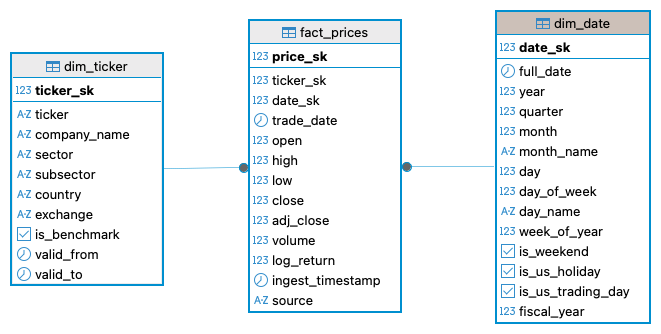
\includegraphics[width=\textwidth]{figures/stocks_er.png}
  \caption{Entity-relationship diagram for the \texttt{stocks} star
    schema, introspected from the live \texttt{dwl-shared-pg} RDS
    instance. The central fact \texttt{stocks.fact\_prices} carries
    the deterministic surrogate \texttt{price\_sk} and two foreign
    keys: \texttt{ticker\_sk} to the SCD~Type~2 ticker dimension and
    \texttt{date\_sk} to the conformed \texttt{analytics.dim\_date}
    dimension. The cross-schema FK to \texttt{analytics.dim\_date}
    is what allows the cross-domain marts in
    Section~6.2 to join stocks against oil and
    news events on the same trading calendar.}
  \label{fig:stocks_er}
\end{figure}

\subsubsection{Oil Schema (S2)}
\label{sec:oil_schema}
The table \texttt{oil.fact\_prices} contains one record per oil type and trading day. The \texttt{oil\_type} attribute distinguishes between Brent and WTI prices, while \texttt{date\_sk} provides a consistent join key to the shared \texttt{analytics.dim\_date} dimension.

\begin{lstlisting}[language=SQL,caption={Oil fact table.},label={lst:oil_schema}]
CREATE TABLE oil.fact_prices (
  price_sk BIGINT PRIMARY KEY,
  date_sk INTEGER NOT NULL REFERENCES analytics.dim_date(date_sk),
  trade_date DATE NOT NULL,
  price NUMERIC,
  oil_type VARCHAR,
  ingest_timestamp TIMESTAMP,
  source VARCHAR
);
\end{lstlisting}

The grain of the table is one observation per oil benchmark and trading day. The \texttt{oil\_type} attribute distinguishes between Brent and WTI prices, while \texttt{date\_sk} provides a consistent join key to the shared \texttt{analytics.dim\_date} dimension. This schema supports historical trend analysis and enables direct comparison of oil prices with stock market and conflict-event data.

\subsubsection{News Events Schema (S3)}
\label{sec:news_schema}

The news domain uses two lake schemas. Silver keeps one row per
normalised Gemini event and intentionally applies no analytical
filtering, so the curated layer remains auditable against the raw JSON.
Its fields are \texttt{event\_date}, \texttt{event\_category},
\texttt{event\_summary}, \texttt{severity},
\texttt{date\_confidence}, \texttt{actors}, \texttt{location},
\texttt{description}, \texttt{source\_hint}, \texttt{url\_hash}, and
\texttt{ingest\_period}. The silver path is
\path{s3://dwl-datapowerchords-curated/news/events_parquet/year=\textless{}YYYY\textgreater{}/month=\textless{}MM\textgreater{}/data.parquet}.

Gold changes the grain to one row per calendar day for joining with
oil, stock, and date dimensions. It excludes approximate-date records
and severity-1 routine records, then writes daily aggregates to
\path{s3://dwl-datapowerchords-gold/news/fact_conflict_daily/event_date=\textless{}YYYY-MM-DD\textgreater{}/data.parquet}.
The gold schema contains the daily event count, maximum and average
severity, conflict flag, top event summary and category, deterministic
\texttt{category\_sk} and \texttt{severity\_sk}, per-category counts
and maximum severities, a \texttt{hormuz\_flag}, and
\texttt{approximate\_count}. This produces the daily conflict-intensity
fact used by the Q1, Q3, and Q4 dashboards.

\subsubsection{Analytics Schema (S1 + S3)}
\label{sec:analytics_schema}

The \texttt{analytics} schema hosts a conformed \texttt{dim\_date}
dimension (owned by S1) and three cross-domain marts used by the
Tableau dashboards. The first mart is the basic daily time series that
aligns all three analytical domains: oil prices, stock returns, and
conflict-event intensity on the shared date dimension. The second mart
adds event-window features around conflict days, so dashboards can
compare pre-event and post-event movement over a consistent horizon.
The third mart aggregates category impact at one row per ticker and
top event category, adding the statistical measures used to rank which
event types had the strongest equity-market effect.

\paragraph{\texttt{dim\_date} (shipped 2026-05-06).}
The dimension covers 2025-01-01 through 2030-12-31 (approximately
2{,}191 calendar days) and was generated once by
\texttt{stocks/sql/migrations/002\_dim\_date\_seed.py}. The script
uses the \texttt{pandas\_market\_calendars}
library for the NYSE calendar, which
handles Good Friday and half-day closures correctly, and the
\texttt{holidays} Python package for US
federal holidays. The output is a single 33.5\,KB
Snappy-compressed Parquet at
\path{s3://dwl-datapowerchords-gold/analytics/dim_date/dim_date.parquet},
registered in the Glue Catalog as
\texttt{analytics\_gold\_dim\_date}. Athena counts at registration
time: 1{,}505 trading days and 80 non-trading-day holidays
(\texttt{is\_us\_holiday=true}) over the 6-year window. The integer
key \texttt{date\_sk} = \texttt{YYYYMMDD} (e.g. \texttt{20260423}) is
the conformed join target referenced by every fact and mart in the
warehouse. Because the dimension is small and stable, no partitioning
is applied; Athena always reads the whole 33.5\,KB file. The
warehouse load step copies these rows into the RDS table
\texttt{analytics.dim\_date} via either a direct
\texttt{INSERT \dots SELECT} from a temporary table or the
\texttt{aws\_s3} PostgreSQL extension, depending on which path proves
cleaner at implementation time.

\newpage
% ======================================================================
% SECTION 5 — DATA TRANSFORMATION
% Primary author: S3
% Contributors:   S1 (stocks subsection), S2 (oil subsection)
% ======================================================================

\section{Data Transformation}
\label{sec:data_transformation}

The transformation layer converts raw API payloads into
analytics-ready Parquet and finally into the RDS star schema. Three
stages apply across all domains: bronze $\to$ silver (parsing,
normalization, PyArrow schema enforcement), silver $\to$ gold
(grouping, partitioning), and gold $\to$ RDS (idempotent upsert).

\subsection{Transformation Logic}
\label{sec:transformation_logic}

\subsubsection{Stocks (S1)}
\label{sec:stocks_transform}

The stocks transform Lambda
(\texttt{dwl-stocks-transform}, Python~3.11, x86\_64, 1024\,MB,
5-minute timeout, layer \texttt{dwl-stocks-deps:1}) reads the latest
bronze JSON per ticker, normalises the field names into the silver
schema, computes the daily log return
$r_t = \ln(P_t / P_{t-1})$ where $P$ is \texttt{adj\_close} following
standard practice in financial econometrics~[7] (the
first row of each ticker's series has \texttt{log\_return = NULL}
because no prior price exists), and writes both the per-ticker
monthly silver Parquet and the per-trade-date gold Parquet. Three
event modes are supported: an empty payload \texttt{\{\}} performs a
daily incremental refresh against the latest bronze partition; a
pinned payload \texttt{\{"ingest\_date":"YYYY-MM-DD"\}} replays from
a specific bronze snapshot (used once on first deploy with the
initial backfill date and otherwise reserved for disaster recovery);
and a
restricted-tickers payload supports targeted smoke testing.

\paragraph{Silver writes are merged, not overwritten.}
Each \texttt{(symbol, year, month)} silver Parquet file is
read-modified-written rather than blindly overwritten: the handler
reads any existing object at the target key, drops the rows whose
\texttt{trade\_date} falls within the new batch (last-write-wins
per date), appends the new rows, sorts, and writes back. Without
this merge step, a routine 7-day-window invocation in the middle of
a month would silently replace that month's silver file with only
those 5--7 trading days, losing all earlier history for the same
month. The merge adds one additional \texttt{S3:GetObject} per file
per run ($\sim$255 GETs across the universe, total cost a few US
cents per month) and preserves the file as the union of all bronze
data ever transformed into it. A full backfill (pinned to the initial
ingest snapshot containing 333 trading days) writes 255 silver files
in approximately 10 seconds; a routine \texttt{\{\}} run overwrites
only the current and previous months and runs in approximately
3 seconds.

\paragraph{Gold writes assemble all 15 tickers per partition.}
After all 15 silver DataFrames are built, the handler concatenates
them and groups by \texttt{trade\_date}, writing a single Parquet
file per date containing 15 rows (one per ticker, sorted by
\texttt{ticker\_sk}). The partition path
\texttt{trade\_date=<YYYY-MM-DD>/part-0000.parquet} aligns with the
Q2 divergence-analysis access pattern (``all tickers for a date
range''), which dominates the Q1 and Q2 dashboards.

\paragraph{Schema constraints surfaced during T5 verification.}
Two AWS Glue and Athena constraints surfaced during operational
verification shape the write logic and are worth flagging as
concrete data-lake idiosyncrasies. First, the Hive table descriptor
rejects ``duplicate columns'' if a column name appears both as a
Parquet field and as a partition key. The handler
therefore drops \texttt{symbol} from the silver Parquet body and
\texttt{trade\_date} from the gold Parquet body before serialising.
Second, Glue Crawlers infer partition-key types as
\texttt{varchar} even when the source Parquet uses the
\texttt{date32} logical type. Athena queries that compare partition
keys to \texttt{DATE} literals therefore require an explicit
\texttt{CAST(trade\_date AS DATE)}. Both constraints disappear at
the RDS load stage (Section~6) because
PostgreSQL columns are strongly typed at create
time. This asymmetry between the data-lake and
warehouse representations is one of the concrete trade-offs the
project surfaces. It is discussed further in the Conclusions
(Section~8).

\subsubsection{Oil (S2)}
\label{sec:oil_transform}
The oil transform Lambda \texttt{dwl-oil-transform} reads the raw JSON responses retrieved from the EIA API and converts them into structured datasets for the silver and gold layers. The transformation process standardises the schema across Brent and WTI observations, converts date fields into a consistent format, and extracts the benchmark identifier and daily price values required for downstream analysis.

For the silver layer, the transformed data is stored as Parquet files partitioned by year and month. This representation preserves the full historical dataset while providing an efficient format for querying and analytical processing. The silver layer serves as the curated representation of the original EIA data and remains closely aligned with the source records.

For the gold layer, the data is transformed into the final analytical schema used by the warehouse and dashboards. Each record represents a single benchmark price observation for a given trading day. Additional attributes such as \texttt{date\_sk} are generated to support integration with the shared \texttt{analytics.dim\_date} dimension and enable cross-domain analysis with stock-market and conflict-event datasets.

The transformation process is implemented as an AWS Lambda function and is triggered automatically after successful ingestion. The resulting Parquet datasets are written to the curated and gold S3 buckets and registered in the AWS Glue Data Catalog. This architecture enables efficient querying through Amazon Athena and supports the subsequent warehouse loading process described in Section~6.

\subsubsection{News and Events (S3)}
\label{sec:news_transform}

The news pipeline has three Lambdas. The ingest Lambda
\texttt{dwl-conflict-ingest} calls Gemini 2.5 Flash with Google Search
grounding, validates that each returned event belongs to the allowed
taxonomy and has severity in the range 1--5, adds an
\texttt{url\_hash} computed from \texttt{event\_date} and
\texttt{event\_summary}, and writes one raw JSON object per
\texttt{event\_date}. Empty days are also written so downstream jobs
can distinguish ``no events'' from ``missing partition''.

The transform Lambda \texttt{dwl-news-transform} performs two
conversions. For silver, it reads all bronze JSON files in each month,
coerces dates, converts actor arrays into comma-separated strings, and
writes Snappy-compressed Parquet with the strict PyArrow schema. For
gold, it reads each day independently, drops approximate-date events
and severity-1 routine events, aggregates the remaining records into a
single daily row, derives category counts and maximum severities, and
sets a Hormuz-related flag when the location or summary mentions
Hormuz, the Strait, the Persian Gulf, or the Red Sea.

The gold daily Parquet output is the handoff point to the warehouse load stage. Loading into RDS is handled by \texttt{dwl-news-load} and is described with the warehouse schema in Section~6.

\begin{figure}[H]
  \centering
  \resizebox{\textwidth}{!}{%
  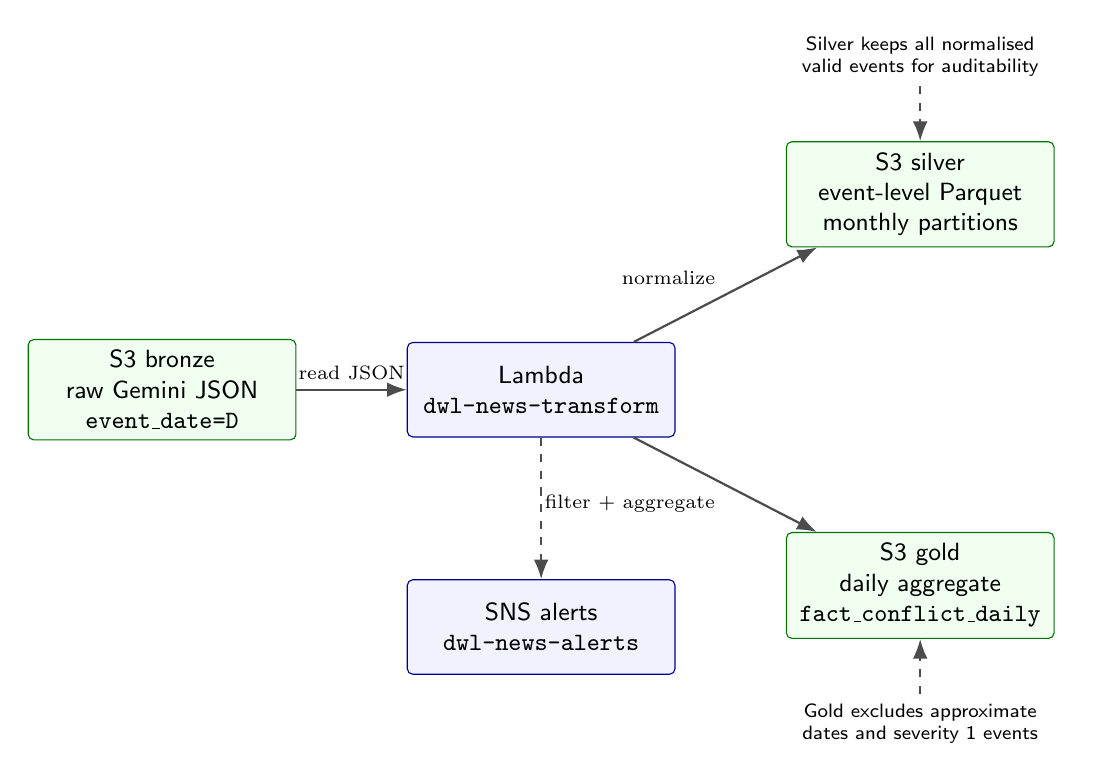
\begin{tikzpicture}[
    font=\sffamily\small,
    node distance=12mm and 14mm,
    box/.style={
      draw,
      rounded corners=2pt,
      align=center,
      minimum width=34mm,
      minimum height=12mm,
      inner sep=4pt,
      fill=white
    },
    aws/.style={
      box,
      fill=blue!5,
      draw=blue!55!black
    },
    data/.style={
      box,
      fill=green!6,
      draw=green!45!black
    },
    db/.style={
      cylinder,
      draw=purple!55!black,
      fill=purple!6,
      shape border rotate=90,
      aspect=0.25,
      align=center,
      minimum width=32mm,
      minimum height=15mm,
      inner sep=4pt
    },
    note/.style={
      align=center,
      font=\sffamily\scriptsize,
      text width=39mm
    },
    arrow/.style={
      -{Latex[length=2.5mm]},
      thick,
      draw=black!70
    }
  ]

    % Main transformation pipeline
    \node[data] (bronze) {S3 bronze\\raw Gemini JSON\\\texttt{event\_date=D}};
    \node[aws, right=of bronze] (transform) {Lambda\\\texttt{dwl-news-transform}};
    \node[data, above right=of transform] (silver) {S3 silver\\event-level Parquet\\monthly partitions};
    \node[data, below right=of transform] (gold) {S3 gold\\daily aggregate\\\texttt{fact\_conflict\_daily}};

    % Support
    \node[aws, below=18mm of transform] (sns) {SNS alerts\\\texttt{dwl-news-alerts}};

    % Arrows
    \draw[arrow] (bronze) -- node[above, font=\scriptsize] {read JSON} (transform);
    \draw[arrow] (transform) -- node[above left, font=\scriptsize] {normalize} (silver);
    \draw[arrow] (transform) -- node[below left, font=\scriptsize] {filter + aggregate} (gold);

    \draw[arrow, dashed] (transform) -- (sns);

    % Notes
    \node[note, above=7mm of silver] (silvernote)
      {Silver keeps all normalised valid events for auditability};
    \draw[arrow, dashed] (silvernote) -- (silver);

    \node[note, below=7mm of gold] (goldnote)
      {Gold excludes approximate dates and severity 1 events};
    \draw[arrow, dashed] (goldnote) -- (gold);

  \end{tikzpicture}%
  }
  \caption{News event transformation from bronze JSON to silver and gold Parquet.}
  \label{fig:news_transform}
\end{figure}



\subsection{Data Cleaning \& Preparation}
\label{sec:data_cleaning}

\paragraph{Missing values.}
Stock rows with a missing \texttt{close} are rejected at silver
write. Oil-price gaps on weekends and US holidays are represented as
row absence rather than forward-filled.

\paragraph{Outliers.}
Sanity-bound checks reject stock rows where \texttt{adj\_close/close}
is outside $[0.1, 10]$.

\paragraph{Duplicates.}
Deterministic S3 key paths for bronze; UPSERT keyed on natural
uniques for gold $\to$ RDS.

\paragraph{Standardisation.}
Timestamps in UTC; prices in \texttt{NUMERIC(18,6)}; booleans as
\texttt{BOOLEAN}.

\subsection{Data Quality \& Validation}
\label{sec:data_quality}

Post-load quality assertions are enforced by a reusable SQL library,
covering uniqueness, completeness, range, referential integrity, and
timeliness. Each domain's Step Functions state machine calls a
quality-check Lambda; violations publish to SNS.

\paragraph{Monitoring.}
Row-count deltas emitted to CloudWatch custom metrics; a 50\% drop
triggers an alarm.

\subsection{Scalability \& Reusability}
\label{sec:scalability}

Three architectural choices support scalability: modular Lambda
structure, shared Python layer, reusable parameterised SQL QA
library. Scaling to hundreds of tickers would use Step Functions Map
state for fanout; heavy transforms would migrate to AWS Glue if
individual Lambda runtime exceeded the 15-minute cap.

\newpage
% ======================================================================
% SECTION 6 — DATA WAREHOUSE
% Primary author: S2
% Contributors:   S1 (stocks star schema), S3 (news_events)
% ======================================================================

\section{Data Warehouse}
\label{sec:data_warehouse}

\subsection{Business Goals and Objectives}
\label{sec:dw_goals}

\paragraph{Stakeholders.}
Geopolitical risk analysts and commodity traders.

\paragraph{Required metrics.}
Daily and rolling-window log-returns per ticker and subsector; daily
WTI/Brent spot and spread; event counts by category; cross-domain
joins aligning stocks, oil, and events on the shared trading day;
event-window pre/post deltas.

\paragraph{Granularity.}
Daily. Intraday rejected given API free-tier limits and because the
research questions operate on daily aggregates.

\subsection{Data Warehouse Modelling (S1)}
\label{sec:dw_modelling}

The data warehouse implements a Kimball-style star
schema~[1]. Each domain owns its own Postgres schema,
and the \texttt{analytics} schema hosts the conformed
\texttt{dim\_date} table and the three cross-domain marts.

\begin{table}[H]
  \centering
  \caption{Facts and dimensions.}
  \label{tab:dw_facts_dims}
  \small
  \begin{tabularx}{\textwidth}{l l X}
    \toprule
    \textbf{Schema} & \textbf{Table} & \textbf{Grain} \\
    \midrule
    \texttt{stocks}      & \texttt{fact\_prices}   & one row per ticker per trading day \\
    \texttt{stocks}      & \texttt{dim\_ticker}    & SCD Type 2 per ticker \\
    \texttt{oil}         & \texttt{fact\_prices}   & one row per series per posting day \\
    \texttt{news\_events}& \texttt{fact\_conflict\_daily} & one row per calendar day \\
    \texttt{news\_events}& \texttt{dim\_event\_category} & 5 event categories \\
    \texttt{news\_events}& \texttt{dim\_severity}  & 1--5 severity scale \\
    \texttt{analytics}   & \texttt{dim\_date}      & per calendar date 2025--2030 \\
    \texttt{analytics}   & \texttt{mart\_daily\_signals}     & calendar day $\times$ ticker, raw joined oil/stock/conflict signals \\
    \texttt{analytics}   & \texttt{mart\_conflict\_sessions} & calendar day $\times$ ticker, session-enriched with forward-filled oil prices \\
    \texttt{analytics}   & \texttt{mart\_category\_impact}   & top event category $\times$ ticker, aggregated return statistics \\
    \bottomrule
  \end{tabularx}
\end{table}

\paragraph{Surrogate keys.}
Surrogate keys are \emph{deterministic} rather than database-issued.
Each fact row's primary key is computed at transform time as a
function of its natural-key components. For stocks the formula is
\texttt{price\_sk} = \texttt{ticker\_sk}~$\times$~$10^9$~+~\texttt{date\_sk},
where \texttt{date\_sk} is the integer \texttt{YYYYMMDD}
representation of the trade date. The $10^9$ multiplier exceeds any
realistic \texttt{date\_sk} value (e.g., $20301231 < 10^9$), so
collisions are impossible. Two consequences flow from this choice.
First, the gold Parquet zone in S3 carries the same surrogate values
that will end up in RDS, so the load Lambda's \texttt{INSERT \dots ON
CONFLICT (price\_sk) DO UPDATE} upsert is fully idempotent. Re-loading
a partition produces no row-count drift, and a partial-failure retry
is a no-op for the rows that already landed. Second, the dimension
seed script
\texttt{stocks/sql/migrations/005\_dim\_ticker\_seed.sql} explicitly
assigns \texttt{ticker\_sk} values 1--15 in the D2 universe order,
matching a static \texttt{TICKER\_SK\_MAP} baked into the transform
Lambda. This pairing is a deliberate contract between the lake and
the warehouse, and it removes the need for any sequence-coordination
protocol between the two storage systems.

\paragraph{Hierarchies.}
Ticker: sector $\to$ subsector $\to$ ticker. Date: year $\to$ quarter
$\to$ month $\to$ day.

\paragraph{Denormalisation of the oil series identifier.}
The oil fact table omits a separate \texttt{dim\_series} dimension and
instead carries the EIA series identifier as a string column directly
on \texttt{oil.fact\_prices}. The choice is deliberate. The series
cardinality is low (WTI, Brent, and a small set of related EIA product
codes), the values are stable across the analysis window, and the
identifier carries no descriptive attributes beyond the code itself
that would justify a dedicated dimension table. The Kimball
dimensional-modelling framework cited in
Section~4.3 explicitly endorses storing
low-cardinality, attribute-poor enumerations directly on the fact
when a full dimension would add no analytical value. As a consequence
the gold-zone catalog also omits \texttt{oil\_gold\_dim\_series},
which keeps the planned cross-domain join surface concentrated on the
conformed \texttt{analytics.dim\_date} dimension that every fact
already shares.

\subsubsection{Stocks Star Schema Contribution (S1)}
\label{sec:dw_stocks}

The stocks portion of the warehouse comprises three tables across two
schemas: \texttt{stocks.fact\_prices} and \texttt{stocks.dim\_ticker}
in the per-domain \texttt{stocks} schema, and the conformed
\texttt{analytics.dim\_date} (owned by S1 but accessed by every
domain) in the shared \texttt{analytics} schema. All three were
provisioned via DDL migrations checked into
\texttt{stocks/sql/migrations/} (\texttt{001\_init\_analytics.sql},
\texttt{004\_init\_stocks.sql}, and the seed scripts
\texttt{003\_dim\_date\_load.py} and
\texttt{005\_dim\_ticker\_seed.sql}) and applied to
\texttt{dwl-shared-pg} via \texttt{psql} in AWS CloudShell. The
schema itself was already shown in
Listing~1 (Section~4.3.1);
this subsection focuses on the \emph{load} chain that populates the
warehouse tables from gold Parquet.

\paragraph{Load Lambda design.}
\texttt{dwl-stocks-load} (Python~3.11, x86\_64, 1024\,MB, 5-minute
timeout) runs on AWS Lambda and reads gold-zone Parquet files at
\path{s3://dwl-datapowerchords-gold/stocks/fact_stock_prices/trade_date=<D>/part-0000.parquet}.
The handler re-injects the \texttt{trade\_date} column (which is
encoded in the S3 path rather than the Parquet body to avoid the
Hive duplicate-column rule) and bulk-inserts via the
\texttt{psycopg2.extras.execute\_values} helper. The connection uses
\texttt{sslmode=require}, which is required because the shared RDS
instance is configured with \texttt{rds.force\_ssl=1}. The master
credentials are fetched at cold-start time from AWS Secrets Manager.

\paragraph{Idempotent UPSERT.}
The insert SQL is:
\begin{lstlisting}[language=SQL,caption={Idempotent UPSERT keyed on the deterministic surrogate.},label={lst:stocks_upsert}]
INSERT INTO stocks.fact_prices (
  price_sk, ticker_sk, date_sk, trade_date,
  open, high, low, close, adj_close, volume,
  log_return, ingest_timestamp, source
) VALUES %s
ON CONFLICT (price_sk) DO UPDATE SET
  open = EXCLUDED.open, high = EXCLUDED.high, ...
\end{lstlisting}
Because \texttt{price\_sk} is deterministic, re-running the load
against an already-loaded partition produces no row count change and
no duplicate-key errors. This idempotency property lets the planned
Step Functions orchestration retry transient failures without
sentinel-row tracking.

\paragraph{Four event modes.}
The handler dispatches on the invocation event. The default empty
payload \texttt{\{\}} loads the previous day's partition and is what
the \texttt{dwl-stocks-load-daily-2210utc} EventBridge Scheduler fires
on weeknights. A \texttt{\{"trade\_date": "YYYY-MM-DD"\}} payload
loads a single explicit partition and is used for smoke tests and
gap-filling. A \texttt{\{"trade\_dates": [...]\}} payload loads a
list of partitions in sequence. Finally, \texttt{\{"backfill": true\}}
lists every gold \texttt{trade\_date} prefix in S3 and loads each in
turn. The backfill mode was used once on first deploy and produced
335 partitions and 5{,}025 rows in approximately two minutes of
wall-clock time.

\paragraph{Daily orchestration.}
Three independent EventBridge schedules currently run the full
pipeline nightly: 22:00\,UTC ingest writes bronze JSON; 22:05\,UTC
transform writes silver and gold Parquet; 22:10\,UTC load upserts
into RDS. A 5-minute offset is sufficient because each upstream stage
runs in well under a minute warm. These three schedules are planned
to be folded into a single Step Functions state machine
\texttt{dwl-stocks-daily} once the orchestration consolidation step
is reached, so that a transform failure short-circuits the load and a
single CloudWatch alarm covers the whole pipeline.

\paragraph{Warehouse-load implementation evidence (verified 2026-05-07).}
End-to-end, the chain populates \texttt{stocks.fact\_prices} with
5{,}025 rows spanning 335 distinct \texttt{trade\_date} values and
all 15 tickers. The SCD2 dimension \texttt{stocks.dim\_ticker}
contains 15 current rows (\texttt{valid\_to IS NULL}) with
\texttt{ticker\_sk} values 1--15 matching the
\texttt{TICKER\_SK\_MAP} contract. The conformed
\texttt{analytics.dim\_date} contains 2{,}191 rows. A representative
star-join verification, shown in
Listing~3, returns five rows for the trading
week of 2026-04-27, with non-null \texttt{close} and
\texttt{log\_return} values on every row, demonstrating that both
foreign keys resolve and the dimensional joins work end-to-end.
\begin{lstlisting}[language=SQL,caption={Star-join verification across the three tables.},label={lst:stocks_starjoin}]
SELECT t.ticker, d.full_date, f.close, f.log_return
FROM   stocks.fact_prices f
JOIN   stocks.dim_ticker  t USING (ticker_sk)
JOIN   analytics.dim_date d USING (date_sk)
WHERE  t.ticker = 'XOM'
  AND  d.full_date BETWEEN DATE '2026-04-27' AND DATE '2026-05-01'
ORDER  BY d.full_date;
\end{lstlisting}
This is the canonical query shape that the cross-domain marts in
Section~6.2 extend with the oil and news
fact-table joins.

\subsubsection{Oil Star Schema Contribution (S2)}
\label{sec:dw_oil}
% TODO S2: mirror the structure of \S~\ref{sec:dw_stocks}.
% Cover: oil.fact_prices grain and columns (including the denormalised
% series identifier per the modelling-section decision), the
% dwl-oil-load Lambda design, idempotent UPSERT keyed on the natural
% unique, daily orchestration, and implementation evidence (row counts,
% star-join verification against analytics.dim_date).
\lipsum[20-21]

\subsubsection{News Events Schema Contribution (S3)}
\label{sec:dw_news}

The warehouse representation for S3's domain is
\texttt{news\_events.fact\_conflict\_daily}. Its fact grain is one
calendar day, matching the gold Parquet grain and the shared
\texttt{analytics.dim\_date} dimension. The load Lambda inserts
\texttt{date\_sk}, \texttt{event\_date}, \texttt{event\_count},
\texttt{max\_severity}, \texttt{avg\_severity},
\texttt{has\_conflict}, \texttt{top\_event\_summary},
\texttt{top\_event\_category}, \texttt{category\_sk},
\texttt{severity\_sk}, five per-category counts, five per-category
maximum severities, \texttt{hormuz\_flag},
\texttt{approximate\_count}, and \texttt{ingest\_timestamp}. The
primary idempotency key is \texttt{event\_date}; reruns update the
same daily row rather than appending a second version.

  For the news domain, \texttt{dwl-news-load} reads the gold Parquet file
  at
  \path{s3://dwl-datapowerchords-gold/news/fact_conflict_daily/event_date=<YYYY-MM-DD>/data.parquet},
  retrieves RDS credentials from Secrets Manager, looks up the conformed
  \texttt{date\_sk} in \texttt{analytics.dim\_date}, and upserts the row
  into \texttt{news\_events.fact\_conflict\_daily}. This keeps the lake
  and warehouse grains identical while allowing failed dates to be
  rerun independently.

Two small dimensions support the fact table. The event-category
dimension maps \texttt{military\_conflict}, \texttt{sanctions},
\texttt{security\_incidents}, \texttt{nuclear\_diplomacy}, and
\texttt{diplomatic\_shifts} to stable surrogate keys. The severity
dimension maps the 1--5 scale to business labels from routine through
extreme. This design avoids storing one row per Gemini event in RDS;
the event-level detail remains in silver Parquet, while the warehouse
keeps the daily aggregate needed by Tableau and cross-domain joins.

\subsubsection{Analytics Mart Contribution (S3)}
\label{sec:dw_analytics_marts}

The final Tableau layer uses three analytics marts. The daily
time-series mart is the broadest table: one row per date, with oil
price measures, benchmark and ticker returns, and the daily conflict
measures from \texttt{news\_events.fact\_conflict\_daily}. It is the
base source for overview charts because every measure shares the same
calendar grain.

The event-window mart reshapes the same data around conflict days. For
each relevant event date it stores market movement before and after
the event, for example same-day, one-day, three-day, and five-day
post-event return windows. This mart supports the Q1 dashboard because
it turns a raw time series into event-study observations.

The category-impact mart is aggregated one level further. Its grain is
one row per ticker and top event category, where the category is taken
from the daily conflict fact's \texttt{top\_event\_category}. It
stores statistical measures such as observation count, average
post-event return, average absolute move, maximum drawdown or
equivalent downside measure, and rank fields used by the Q4 dashboard.
This design keeps the expensive event-window calculations out of
Tableau and gives the workbook compact tables optimised for filtering
and ranking.

\begin{figure}[H]
  \centering
  \resizebox{\textwidth}{!}{%
  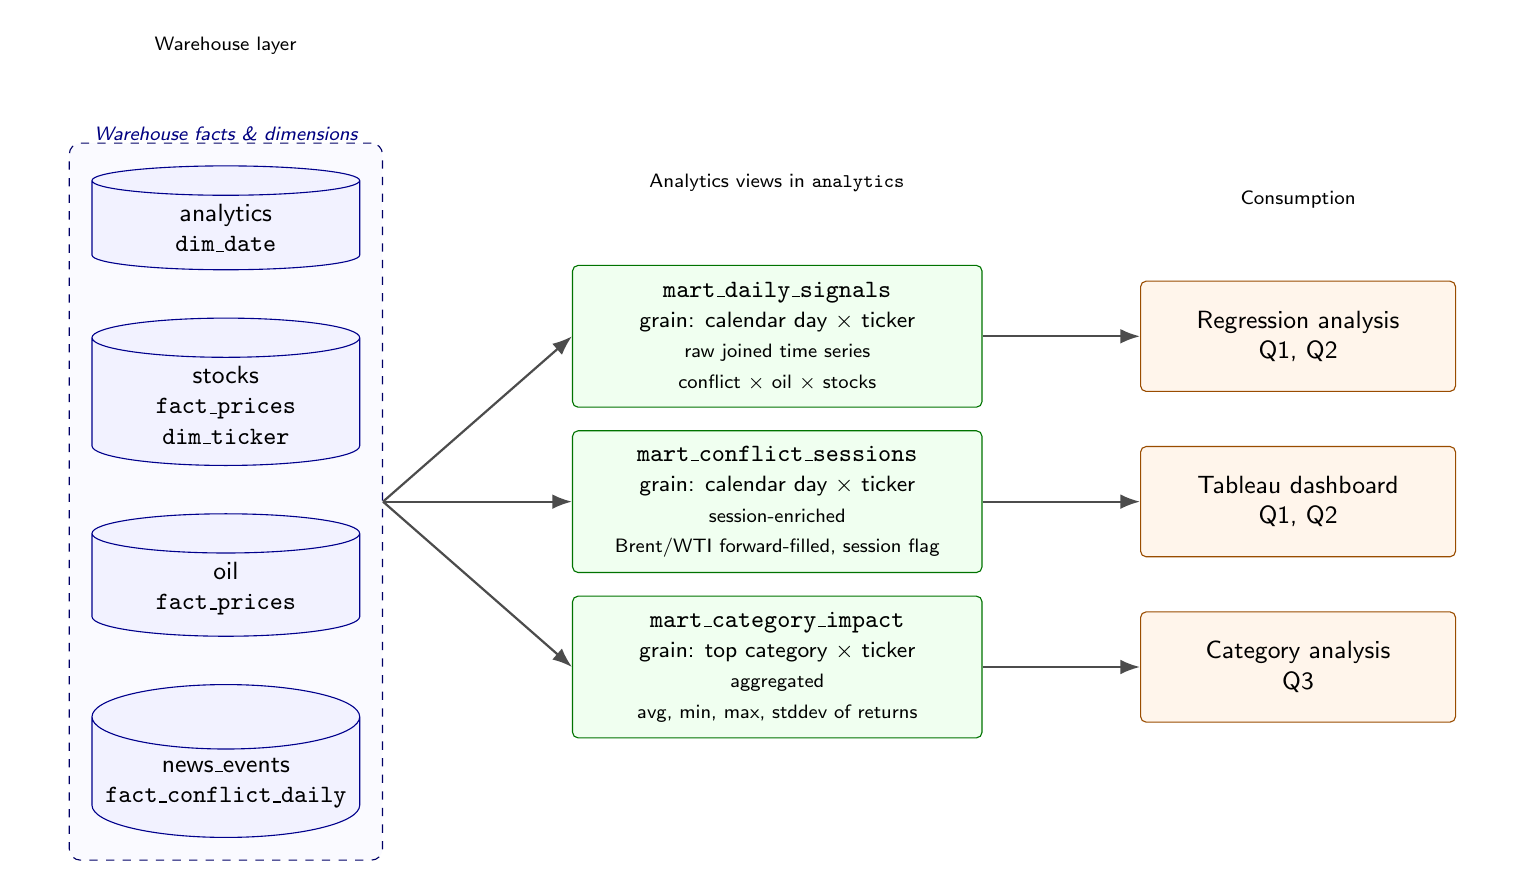
\begin{tikzpicture}[
    font=\sffamily\small,
    node distance=6mm and 16mm,
    source/.style={
      cylinder,
      shape border rotate=90,
      aspect=0.25,
      draw=blue!55!black,
      fill=blue!5,
      align=center,
      minimum width=34mm,
      minimum height=12mm,
      inner sep=3pt
    },
    mart/.style={
      draw,
      rounded corners=2pt,
      fill=green!6,
      draw=green!45!black,
      align=center,
      minimum width=52mm,
      minimum height=18mm,
      inner sep=5pt
    },
    viz/.style={
      draw,
      rounded corners=2pt,
      fill=orange!8,
      draw=orange!60!black,
      align=center,
      minimum width=40mm,
      minimum height=14mm,
      inner sep=4pt
    },
    note/.style={
      align=center,
      font=\sffamily\scriptsize,
      text width=48mm
    },
    arrow/.style={
      -{Latex[length=2.5mm]},
      thick,
      draw=black!70
    }
  ]

    % Warehouse source tables
    \node[source] (date) {analytics\\\texttt{dim\_date}};
    \node[source, below=of date] (stocks) {stocks\\\texttt{fact\_prices}\\\texttt{dim\_ticker}};
    \node[source, below=of stocks] (oil) {oil\\\texttt{fact\_prices}};
    \node[source, below=of oil] (news) {news\_events\\\texttt{fact\_conflict\_daily}};

    % Group source tables into a warehouse cluster (drawn on background layer)
    \begin{scope}[on background layer]
      \node[
        draw=blue!40!black,
        dashed,
        rounded corners=4pt,
        fill=blue!2,
        fit=(date)(stocks)(oil)(news),
        inner sep=8pt,
        label={[font=\sffamily\scriptsize\itshape, blue!50!black, yshift=-1mm]above:Warehouse facts \& dimensions}
      ] (warehouse) {};
    \end{scope}

    % Mart views — vertically centered against the warehouse cluster
    \node[mart, right=24mm of warehouse.east, yshift=21mm] (daily) {\texttt{mart\_daily\_signals}\\
      \footnotesize grain: calendar day $\times$ ticker\\
      \scriptsize raw joined time series\\
      \scriptsize conflict $\times$ oil $\times$ stocks};

    \node[mart, right=24mm of warehouse.east] (sessions) {\texttt{mart\_conflict\_sessions}\\
      \footnotesize grain: calendar day $\times$ ticker\\
      \scriptsize session-enriched\\
      \scriptsize Brent/WTI forward-filled, session flag};

    \node[mart, right=24mm of warehouse.east, yshift=-21mm] (impact) {\texttt{mart\_category\_impact}\\
      \footnotesize grain: top category $\times$ ticker\\
      \scriptsize aggregated\\
      \scriptsize avg, min, max, stddev of returns};

    % Consumption nodes
    \node[viz, right=20mm of daily] (dailyviz) {Regression analysis\\Q1, Q2};
    \node[viz, right=20mm of sessions] (sessionsviz) {Tableau dashboard\\Q1, Q2};
    \node[viz, right=20mm of impact] (impactviz) {Category analysis\\Q3};

    % Warehouse cluster to mart arrows — one per mart
    \draw[arrow] (warehouse.east) -- (daily.west);
    \draw[arrow] (warehouse.east) -- (sessions.west);
    \draw[arrow] (warehouse.east) -- (impact.west);

    % Mart to consumption arrows
    \draw[arrow] (daily.east) -- (dailyviz.west);
    \draw[arrow] (sessions.east) -- (sessionsviz.west);
    \draw[arrow] (impact.east) -- (impactviz.west);

    % Section labels above
    \node[note, above=10mm of warehouse.north] {Warehouse layer};
    \node[note, above=8mm of daily] {Analytics views in \texttt{analytics}};
    \node[note, above=8mm of dailyviz] {Consumption};

  \end{tikzpicture}%
  }
  \caption{Analytics marts implemented as cross-domain SQL views over warehouse facts. Each mart joins all four source tables. \texttt{mart\_daily\_signals} provides the raw joined time series; \texttt{mart\_conflict\_sessions} adds session-window logic and forward-filled oil prices for visualization; \texttt{mart\_category\_impact} pre-aggregates return statistics by conflict category.}
  \label{fig:analytics_marts}
\end{figure}

\subsection{Architecture (S2)}
\label{sec:dw_architecture}

The data warehouse runs on a single shared RDS PostgreSQL 16
\texttt{db.t4g.micro} in \texttt{us-east-1}. The instance is publicly
reachable with TLS enforced via \texttt{rds.force\_ssl}. Four schemas
on one database were chosen over three separate instances for cost
and for simpler cross-schema joins.

\begin{figure}[H]
  \centering
  \fbox{\parbox{0.9\textwidth}{\centering
    \textit{Placeholder. Commit DW architecture diagram.}}}
  \caption{Data warehouse architecture.}
  \label{fig:dw_architecture}
\end{figure}

\subsection{Data Preparation}
\label{sec:dw_data_prep}

\paragraph{Extraction.}
Each domain's load Lambda reads the gold-zone Parquet partition and
streams rows to RDS in a single server-side transaction.

\paragraph{Transformation rules.}
Minimal residual: surrogate-key lookups and NULL-handling.

\paragraph{Loading strategy.}
Incremental. Each day's load Lambda writes only the current partition
via \texttt{INSERT \dots ON CONFLICT \dots DO UPDATE}. Full reloads
never required; bronze preserves all state for replay.

\newpage
% ======================================================================
% SECTION 7 — DATA VISUALIZATION
% Primary author: S3
% Contributors:   S1 (Q1/Q2 answers), S2 (Q1/Q4 answers)
% ======================================================================

\section{Data Visualization}
\label{sec:data_visualization}

\subsection{Visualization Purpose}
\label{sec:viz_purpose}

\paragraph{Problem.}
Expose relationships between conflict events, oil moves, and energy
stocks interactively for a non-technical analyst audience.

\paragraph{Target audience.}
Geopolitical risk analysts and commodity traders.

\paragraph{Decisions supported.}
Event-category effect sizes (BI1), subsector reactivity (BI2),
conflict intensity as volatility indicator (BI3), case-study
deep-dives (BI4).

\subsection{Theoretical Model}
\label{sec:theoretical_model}

The workbook follows Shneiderman's visual-information-seeking mantra:
overview first, zoom and filter, then details-on-demand. The home
dashboard provides the overview; per-research-question dashboards
allow filtering; tooltips and click-through links provide
details-on-demand.

\subsection{Data Warehouse Visualization (S3)}
\label{sec:dw_visualization}

The Tableau workbook contains five dashboards: a home overview plus
one per research question (Q1 event $\to$ oil reaction, Q2 subsector
divergence, Q3 conflict intensity vs volatility, Q4 event-type ranking).

\begin{figure}[H]\centering
  \fbox{\parbox{0.9\textwidth}{\centering\textit{Q1 dashboard placeholder.}}}
  \caption{Q1: event-category reaction distribution.}\label{fig:dash_q1}
\end{figure}

\begin{figure}[H]\centering
  \fbox{\parbox{0.9\textwidth}{\centering\textit{Q2 dashboard placeholder.}}}
  \caption{Q2: rolling cross-ticker correlation heatmap.}\label{fig:dash_q2}
\end{figure}

\begin{figure}[H]\centering
  \fbox{\parbox{0.9\textwidth}{\centering\textit{Q3 dashboard placeholder.}}}
  \caption{Q3: conflict intensity overlaid on idiosyncratic volatility.}\label{fig:dash_q3}
\end{figure}

\begin{figure}[H]\centering
  \fbox{\parbox{0.9\textwidth}{\centering\textit{Q4 dashboard placeholder.}}}
  \caption{Q4: event-type impact ranking.}\label{fig:dash_q4}
\end{figure}

\subsection{Answer to Business Questions}
\label{sec:bq_answers}

\subsubsection{Q1: Conflict events vs oil price spikes (S2 + S3)}
\label{sec:answer_q1}
% TODO S2/S3
\lipsum[24-25]

\subsubsection{Q2: Subsector synchrony vs divergence (S2)}
\label{sec:answer_q2}
% Reassigned from S1 to S2 because S2 owns the Tableau workbook access.
\lipsum[26-27]

\subsubsection{Q3: Conflict-event intensity vs volatility windows (S3)}
\label{sec:answer_q3}
% TODO S3
\lipsum[28-29]

\subsubsection{Q4: Event-type impact ranking (S2 + S3)}
\label{sec:answer_q4}
% TODO S2/S3
\lipsum[30-31]

\newpage
% ======================================================================
% SECTION 8 — CONCLUSIONS
% All three students equal: S1 -> 8.1, S2 -> 8.2, S3 -> 8.3 + 8.4
% Maximum 2 pages per the template.
% ======================================================================

\section{Conclusions}
\label{sec:conclusions}

\subsection{Discussion of the Solution (S1)}
\label{sec:discussion}

\paragraph{Advantages.}
The architecture exploits AWS managed services where they are
strongest. Bronze--silver--gold zones cleanly separate immutable raw
state from analytics-ready state. The tiered 15-ticker universe is
the key analytical choice making the Q2 divergence and Q4 Hormuz
findings possible.

\paragraph{Disadvantages and trade-offs.}
The RDS instance is public-endpoint rather than VPC-isolated, which
is a deliberate trade of defence-in-depth for reduced complexity
given the 6.5-week timeline. Provisioning uses the AWS Console rather
than Infrastructure-as-Code, which accelerated learning at the cost
of reproducibility. The analysis window starts 2025-01-01, which
narrows Q4 event-type diversity. The HSLU sandbox account also
restricts \texttt{aws glue tag-resource} on Glue \emph{table} ARNs;
the call returns a bare \texttt{InvalidInputException} with no
message body, while the same call against database ARNs succeeds.
The team worked around this by applying per-table catalog tags as
Hive \texttt{TBLPROPERTIES} via Athena \texttt{ALTER TABLE}
statements. The functional outcome is that catalog tables visibly
carry \texttt{project=dwl}, \texttt{owner=sN}, and
\texttt{domain=<dom>} fields in the standard catalog metadata format
used for governance and auditability. The workaround nevertheless
illustrates the kind of sandbox-versus-production gap that a
real-world ETL team would typically document in a runbook for future
joiners.

The news domain has an additional source-specific trade-off. Replacing
World News API with Gemini 2.5 Flash and Google Search grounding solved
the historical-depth problem in the free news-API tiers, but it also
introduced model risk: event discovery, category assignment, and
severity scoring are produced by a generative system rather than by a
fixed article feed. The pipeline mitigates this through strict JSON
validation, recorded \texttt{source\_hint} and
\texttt{date\_confidence}, retention of event-level silver records, and
stricter filtering before the gold warehouse fact is built.

\paragraph{Silent failures in EventBridge Scheduler IAM policies.}
A subtler operational lesson surfaced eight days into the
daily-load window after the warehouse-load chain went live. The AWS Console's EventBridge Scheduler wizard,
when invoked with the ``Create new role for this schedule'' option,
generates an inline policy whose \texttt{Resource} array is scoped
narrowly to the single Lambda chosen during creation. When the same role was later
re-used to invoke a second schedule
(\texttt{dwl-stocks-transform-daily-2205utc}) and a third
(\texttt{dwl-stocks-load-daily-2210utc}), the wizard did not prompt
for the resource list to be expanded, and the new schedules silently
failed at the invocation-attempt stage because the role lacked
\texttt{lambda:InvokeFunction} on those Lambdas' ARNs. The failure
was invisible by design. The schedule remained ``Enabled'', its
``Next 10 trigger dates'' panel populated correctly, the target
Lambda's CloudWatch log group simply had no streams for the scheduled
times, and the Lambda's invocation chart showed zero scheduled fires.
Without a configured dead-letter queue or a CloudWatch log group on
the schedule itself (neither is the wizard default), the only
externally observable symptom was the downstream data product
diverging from expectation. The row count in \texttt{stocks.fact\_prices}
stayed at the backfill value of 5{,}025 instead of growing daily.
Diagnosis required tracing the chain from RDS back through the gold
zone (where data was current) to the IAM policy (where it was not),
eventually identifying the missing \texttt{Resource} entries. The
remediation was to expand the policy's \texttt{Resource} array to
the wildcard \texttt{function:dwl-stocks-*}, which is a one-line
change. The
takeaway is that silent failures without log breadcrumbs are an
operational hazard distinct from incorrect data. Future projects
should always attach a dead-letter queue or an explicit log target
to EventBridge Scheduler in production deployments. The planned
consolidation into AWS Step Functions later in the project removes
this entire class of error because the state machine produces visible
state transitions for every step.

\paragraph{Technology trade-offs.}
The stocks ingest was originally specified to use the Alpha Vantage
free tier for its stable API contract, but the chosen
\texttt{TIME\_SERIES\_DAILY\_ADJUSTED} endpoint moved behind a
paywall shortly after the project began. The project pivoted to the
open-source \texttt{yfinance} library, which proved unmetered for the
15-ticker daily-call volume but required attention to its persistent
caches on the read-only Lambda filesystem. A shared
\texttt{db.t4g.micro} was chosen over three private RDS instances to
keep the budget shared and the cross-domain JOINs trivially
expressible. The Glue Data Catalog serves as a metadata registry
across all three S3 zones, and \textbf{both} Athena and RDS are used
as serving layers. Athena queries gold Parquet directly to power the
interim Tableau prototype that de-risked the May~21 presentation, and
RDS became the primary serving layer for sub-second dashboard
interactions once the warehouse loads completed. This dual-path
lake-and-warehouse architecture is the project's clearest
demonstration of why the course title pairs the two paradigms.

\subsection{Project Outcomes (S2)}
\label{sec:outcomes}

% TODO S2: fill in actual outcomes after W5.

\paragraph{Research-question coverage.}
% TODO S2
\lipsum[32]

\paragraph{System metrics.}
% TODO S2: row counts, ingestion reliability, cost summary.
\lipsum[33]

\subsection{Future Work}
\label{sec:future_work}

Directions that would materially strengthen a successor project:

\begin{itemize}
  \item \textbf{VPC-isolated deployment.} Move RDS into private
        subnets, attach load Lambdas to the VPC, use VPC endpoints.
  \item \textbf{Infrastructure-as-Code.} Replace Console runbooks
        with Terraform for reproducibility and change review.
  \item \textbf{Widen the analysis window.} Paid news archive to
        extend coverage back to 2015, tripling event diversity.
  \item \textbf{Intraday granularity around event windows.} A paid
        intraday data feed (e.g.\ Polygon.io, IEX Cloud, or a
        commercial yfinance-compatible source) would give minute-bar
        precision on event reactions; daily bars compress
        same-session moves into a single closing print.
  \item \textbf{Real-time alerting.} Shift news ingest to streaming
        for within-minutes dashboard refresh on high-severity events.
\end{itemize}

\subsection{GenAI Declaration}
\label{sec:genai_declaration}

The project team used generative-AI tools as follows:

\begin{itemize}
  \item \textbf{Google Gemini API} is a functional component of the
        production pipeline: it researches grounded Iran-region
        conflict events and classifies them into the five-category
        event taxonomy. Its outputs are stored in the bronze zone and
        feed directly into the silver event Parquet and
        \texttt{news\_events.fact\_conflict\_daily}.
  \item \textbf{Claude (Anthropic)} was used during planning and
        documentation to structure the team's architecture decisions,
        draft the implementation plan, and generate first-pass LaTeX
        scaffolding for this report. All substantive technical
        content, prose, and analytical findings were written,
        reviewed, and edited by the three team members.
  \item No generative-AI tool was used for the final analytical
        findings, the Tableau visualisations, or the bibliography.
\end{itemize}

\newpage
% ======================================================================
% REFERENCES
% Minimum 10 per the evaluation guidelines.
% Uses thebibliography environment — no BibTeX pass required.
% ======================================================================

\begin{thebibliography}{99}

\bibitem{kimball2013}
Kimball, R., \& Ross, M. (2013).
\emph{The Data Warehouse Toolkit: The Definitive Guide to Dimensional Modeling} (3rd ed.). Wiley.

\bibitem{inmon2005}
Inmon, W. H. (2005).
\emph{Building the Data Warehouse} (4th ed.). Wiley.

\bibitem{armbrust2020}
Armbrust, M., et al. (2020).
Delta Lake: High-Performance ACID Table Storage over Cloud Object Stores.
\emph{Proceedings of the VLDB Endowment}, 13(12), 3411--3424.

\bibitem{shneiderman1996}
Shneiderman, B. (1996).
The Eyes Have It: A Task by Data Type Taxonomy for Information Visualizations.
In \emph{Proceedings of the 1996 IEEE Symposium on Visual Languages}, 336--343.

\bibitem{few2006}
Few, S. (2006).
\emph{Information Dashboard Design: The Effective Visual Communication of Data}. O'Reilly.

\bibitem{mackinlay1997}
MacKinlay, A. C. (1997).
Event Studies in Economics and Finance.
\emph{Journal of Economic Literature}, 35(1), 13--39.

\bibitem{campbell1997}
Campbell, J. Y., Lo, A. W., \& MacKinlay, A. C. (1997).
\emph{The Econometrics of Financial Markets}. Princeton University Press.

\bibitem{caldara2022}
Caldara, D., \& Iacoviello, M. (2022).
Measuring Geopolitical Risk.
\emph{American Economic Review}, 112(4), 1194--1225.

\bibitem{kilian2009}
Kilian, L. (2009).
Not All Oil Price Shocks Are Alike: Disentangling Demand and Supply Shocks in the Crude Oil Market.
\emph{American Economic Review}, 99(3), 1053--1069.

\bibitem{tetlock2007}
Tetlock, P. C. (2007).
Giving Content to Investor Sentiment: The Role of Media in the Stock Market.
\emph{The Journal of Finance}, 62(3), 1139--1168.

\end{thebibliography}

\addcontentsline{toc}{section}{References}

\newpage
% ======================================================================
% APPENDICES
% \appendix switches section numbering from numeric to letters
% ======================================================================

\appendix

\section{Appendix: Supporting Material}
\label{appx:extras}

\subsection{Ticker Universe}
\label{appx:tickers}

\begin{lstlisting}[language=Python,caption={The 15-ticker tiered universe.},label={lst:tickers}]
TICKERS = [
    # Oil majors
    "XOM", "CVX", "SHEL",
    # Exploration & production (upstream)
    "COP", "OXY", "DVN",
    # Refiners (downstream)
    "VLO", "MPC",
    # Oilfield services
    "SLB", "HAL", "BKR",
    # Tanker / shipping (for Q4 Strait of Hormuz)
    "FRO",
    # Benchmarks
    "XLE",  # energy-sector ETF -- for idiosyncratic volatility
    "USO",  # WTI ETF -- market-traded oil proxy
    "SPY",  # S&P 500 ETF -- market control
]
\end{lstlisting}

\subsection{Key Design Choices}
\label{appx:decisions}

A small number of design choices recur throughout the report and are
collected here for convenience. The data sources for the three
domains are Yahoo Finance via the \texttt{yfinance} library for
stocks, the U.S.\ Energy Information Administration's open API for
oil, and Gemini 2.5 Flash with Google Search grounding for conflict
events.
The stock-price source was changed from Alpha Vantage to
\texttt{yfinance} in May 2026 after the relevant Alpha Vantage
endpoint was moved to a premium tier. The instrument universe is
fifteen tickers grouped into integrated majors, exploration and
production, refiners, oilfield services, tanker shipping, and three
benchmark exchange-traded funds. The analysis window starts on
1~January~2025 and extends to the present. All AWS resources are
provisioned in the \texttt{us-east-1} region by direct Console
operations rather than Infrastructure-as-Code, with markdown runbooks
serving as the executable record.

The shared infrastructure consists of three Amazon S3 buckets (raw,
curated, gold), one PostgreSQL~16 RDS instance shared by all three
domains, an AWS Glue Data Catalog database for metadata, and three
per-domain SNS topics for alerting. The RDS instance is reachable
on its public DNS endpoint over TLS; no private VPC is used, on
cost-versus-complexity grounds for the project's timeline. All three
students sign in via the HSLU access portal and assume the same SSO
permission set; per-Lambda execution roles are scoped to one S3
prefix, one Secrets~Manager namespace, one SNS topic, and the
relevant Glue catalog entries.

Each Lambda layer is per-domain rather than shared, because the
combined unzipped size of the dependencies needed by the stocks
ingest function and the stocks transform-and-load functions exceeds
the AWS-imposed 250\,MB layer cap on a single function. The silver
zone of the data lake is written by a merge-not-overwrite strategy
to keep monthly Parquet files complete under daily 7-day-window
incremental runs. Gold-zone fact partitions encode the time key in
the Hive partition path rather than the Parquet body, which avoids
the duplicate-column rule that Hive enforces but introduces a
\texttt{varchar} partition-key typing in Glue Crawlers, requiring an
explicit \texttt{CAST(\dots AS DATE)} in Athena queries that compare
to date literals. Surrogate primary keys in the warehouse are
deterministic functions of natural-key components, computed at
transform time, which makes the load step idempotent under
\texttt{INSERT \dots ON CONFLICT \dots DO UPDATE}. Per-table catalog
tags are applied as Hive \texttt{TBLPROPERTIES} via Athena
\texttt{ALTER TABLE} statements rather than \texttt{aws glue tag-resource},
because the latter returns an unhelpful
\texttt{InvalidInputException} on table ARNs in the HSLU sandbox
account.

\subsection{Gemini Event Extraction Prompt}
\label{app:gemini_prompt}

\begin{lstlisting}[language={},caption={Prompt used for grounded Gemini event extraction.}]
You are a geopolitical intelligence analyst specialising in Iran and Middle East oil-market risk. Research and return the most significant Iran-region geopolitical conflict events that occurred between {start_date} and {end_date} inclusive.

SCOPE
- Primary actor: Iran (including IRGC, Iranian proxies)
- Region: Iran, Iraq, Yemen, Saudi Arabia, UAE, Oman, Israel, Lebanon, Syria, 
Kuwait, Bahrain, Qatar, Strait of Hormuz, Red Sea, Persian Gulf
- Relevant actors: Iran, IRGC, Houthi, Hezbollah, Israel, United States, Saudi Arabia, UAE

CATEGORIES
  sanctions          - Economic/financial pressure tools: sanctions, tariffs, export restrictions.
                       NOT for military actions even if they have economic effects.
  military_conflict  - Direct use of armed force: strikes, battles, raids, cross-border clashes.
                       USE THIS for naval blockades, airstrikes, missile attacks.
  security_incidents - Non-traditional security events: cyberattacks, maritime disruptions, 
tanker seizures, terrorism, sabotage.
  nuclear_diplomacy  - Nuclear programme diplomacy, IAEA inspections, negotiations, escalation signals.
  diplomatic_shifts  - Summits, ceasefires, alliance shifts, normalisation, breakdown of relations.

SEVERITY SCALE (1-5) - follow this scale strictly, do not underrate
  1 - Routine    : diplomatic statement, minor patrol incident, low-level skirmish,
                   routine military posturing, spokesperson comment
                   EXAMPLE: "Iran foreign minister warns against sanctions"
  2 - Notable    : new sanctions package, small-scale drone/missile launch, naval warning,
                   proxy group credible threat, IAEA routine report
                   EXAMPLE: "US sanctions 3 Iranian oil tankers"
  3 - Significant: confirmed airstrike with damage, tanker seizure, major sanctions
                   targeting key sector (oil minister, central bank), IAEA escalation signal
                   EXAMPLE: "US airstrikes kill IRGC commanders in Syria"
  4 - Severe     : major strike campaign with significant casualties, coordinated
                   multi-front attack, direct Hormuz shipping disruption, nuclear
                   enrichment red line crossed
                   EXAMPLE: "Houthi missiles sink commercial vessel in Red Sea"
  5 - Extreme    : direct Iran-US or Iran-Israel military exchange on Iranian soil,
                   naval blockade of Iranian ports, Hormuz closure or blockade,
                   nuclear weapon test or assembly confirmed, regional war declaration
                   EXAMPLE: "US naval blockade of all Iranian ports announced"
                   EXAMPLE: "Israel strikes Iranian nuclear facilities directly"
  IMPORTANT: A naval blockade, Hormuz closure, or direct military strike on Iran = severity 5. Do NOT rate these as 3 or 4. When in doubt between two levels, choose the higher one.

DATE CONFIDENCE
  exact       - confirmed date from a dated news source
  approximate - event is real but exact date uncertain

RULES
- Return only the top {max_events} most significant events for the period.
- Only include events with a clear Iran/proxy connection or direct oil-market relevance.
- Each event maps to exactly one category.
- event_summary must be 8 words or fewer as a compact dashboard tag.
- Only include date_confidence = "exact" unless severity >= 4.
- CRITICAL: If no relevant events occurred, you MUST return an empty JSON array [] and nothing else. Never return prose or explanation.
- Return ONLY a valid JSON array. No markdown fences. No explanation. No backticks.

OUTPUT FORMAT
[
  {{
    "event_date": "YYYY-MM-DD",
    "event_category": "<category>",
    "event_summary": "<compact tag>",
    "severity": <1|2|3|4|5>,
    "date_confidence": "<exact|approximate>",
    "actors": ["actor1", "actor2"],
    "location": "<country or region>",
    "description": "<1 sentence max factual description>",
    "source_hint": "<publication or outlet>"
  }}
]

\end{lstlisting}

\section{Appendix: Project Evaluation Grid}
\label{appx:evaluation_grid}

\begin{table}[H]
  \centering
  \caption{Final Report Evaluation Grid. ``P'' = primary author,
    ``x'' = contributor of a substantive domain-specific subsection.
    All three columns are fully claimed so that each student has
    equal maximum grade potential.}
  \label{tab:evaluation_grid}
  \small
  \begin{tabular}{@{}p{8.5cm} c c c c@{}}
    \toprule
    \textbf{Evaluation Criteria} & \textbf{Max} & \textbf{S1} & \textbf{S2} & \textbf{S3} \\
    \midrule
    \textbf{1. Introduction}                                & 5 & x & P & P \\
    \quad Topic introduction                                &   &   &   &   \\
    \quad Motivation                                        &   &   &   &   \\
    \quad Problem definition and goals                      &   &   &   &   \\
    \quad Business / research questions                     &   &   &   &   \\
    \quad Business intelligence questions                   &   &   &   &   \\
    \addlinespace
    \textbf{2. Data Lake}                                   & 5 & P & x & x \\
    \quad Data assumptions                                  &   &   &   &   \\
    \quad Architecture                                      &   &   &   &   \\
    \addlinespace
    \textbf{3. Data Ingestion (Lake and Warehouse)}         & 5 & x & P & x \\
    \quad Data source documentation                         &   &   &   &   \\
    \quad Pipeline design                                   &   &   &   &   \\
    \quad Data capture and handling                         &   &   &   &   \\
    \addlinespace
    \textbf{4. Data Storage}                                & 5 & P & x & x \\
    \quad Storage layers and services                       &   &   &   &   \\
    \quad Data formats and optimization                     &   &   &   &   \\
    \quad Database design                                   &   &   &   &   \\
    \addlinespace
    \textbf{5. Data Transformation (Lake and Warehouse)}    & 5 & x & x & P \\
    \quad Transformation logic                              &   &   &   &   \\
    \quad Data cleaning and preparation                     &   &   &   &   \\
    \quad Data quality and validation                       &   &   &   &   \\
    \quad Scalability and reusability                       &   &   &   &   \\
    \addlinespace
    \textbf{6. Data Warehouse}                              & 5 & x & P & x \\
    \quad Business goals and objectives                     &   &   &   &   \\
    \quad Data warehouse modelling                          &   &   &   &   \\
    \quad Architecture                                      &   &   &   &   \\
    \quad Data preparation                                  &   &   &   &   \\
    \addlinespace
    \textbf{7. Data Visualization}                          & 5 & x & x & P \\
    \quad Visualization purpose                             &   &   &   &   \\
    \quad Theoretical model                                 &   &   &   &   \\
    \quad Data warehouse visualizations                     &   &   &   &   \\
    \quad Answer business questions                         &   &   &   &   \\
    \addlinespace
    \textbf{8. Conclusions}                                 & 5 & P & P & P \\
    \quad Discussion of the solution                        &   &   &   &   \\
    \quad Discussion of the project outcomes                &   &   &   &   \\
    \quad Future work                                       &   &   &   &   \\
    \quad GenAI declaration                                 &   &   &   &   \\
    \midrule
    \textbf{Total claimed}                                  & \textbf{40} & \textbf{40} & \textbf{40} & \textbf{40} \\
    \bottomrule
  \end{tabular}
\end{table}

\section{Appendix: Project Code Leads}
\label{appx:code_leads}

\begin{table}[H]
  \centering
  \caption{Code-ownership assignments. X indicates primary responsibility.}
  \label{tab:code_leads}
  \small
  \begin{tabularx}{\textwidth}{@{} X c c c @{}}
    \toprule
    \textbf{Responsibility} & \textbf{S1} & \textbf{S2} & \textbf{S3} \\
    \midrule
    Introduction (already drafted)                                     &    & X  & X  \\
    API Data Source 1 (yfinance, stocks)                               & X  &    &    \\
    API Data Source 2 (EIA, oil)                                       &    & X  &    \\
    API Data Source 3 (Gemini grounded conflict events)                            &    &    & X  \\
    Ingest / Transform / Load Lambdas (per domain)                     & X  & X  & X  \\
    Step Functions + EventBridge (per domain)                          & X  & X  & X  \\
    RDS schema + migrations (per domain)                               & X  & X  & X  \\
    Shared infrastructure provisioning (S3, RDS, Glue DB, IAM, SNS)    & X  &    &    \\
    Team Infrastructure Contract document                              & X  &    &    \\
    AWS Console runbooks                                               & X  &    &    \\
    \texttt{analytics.dim\_date} (shared trading calendar)             & X  &    &    \\
    Top-level repository README, \texttt{DECISIONS.md}                 & X  &    &    \\
    GitHub repository creation + admin                                 &    & X  &    \\
    \texttt{analytics.*} cross-domain mart tables                      &    &    & X  \\
    SQL data-quality library (shared, reusable)                        &    & X  &    \\
    Tableau workbook                                                   &    &    & X  \\
    Jupyter exploration notebooks (per domain)                         & X  & X  & X  \\
    \bottomrule
  \end{tabularx}
\end{table}

\end{document}
